%\chapter{\Objectivethreename}
\chapter[Interpretable Regularized Kernel Cross-Spectral FC Network]{IRKCS-FCnet: Interpretable Regularized Kernel Cross-Spectral Functional Connectivity Network with Qualitative and Quantitative Post-Hoc and Intrinsic Explainability}\label{chapter_3}

In this chapter, we introduce an Interpretable Regularized Kernel Cross-Spectral FC network, named IRKCS-FCnet, as depicted in \cref{fig:contribution3}. This approach minimizes spurious connectivities by optimizing Renyi's entropy of KCS-FC matrices. Both IRKCS-FCnet and its plain version, KCS-FCnet, deploy a CNN layer to extract temporal-spectral features for enhanced FC estimation. The performance of our proposed approach is assessed employing both post-hoc and intrinsic quantitative and qualitative strategies, and it is compared against EEGnet, the recognized standard. While achieving notable accuracy, the IRKCS-FCnet also produces improved interpretable FC matrices. Overall, our results demonstrate that our model architecture achieves comparable MI classification while improving the transparency and interoperability.

\begin{figure}[h!]
    \centering
    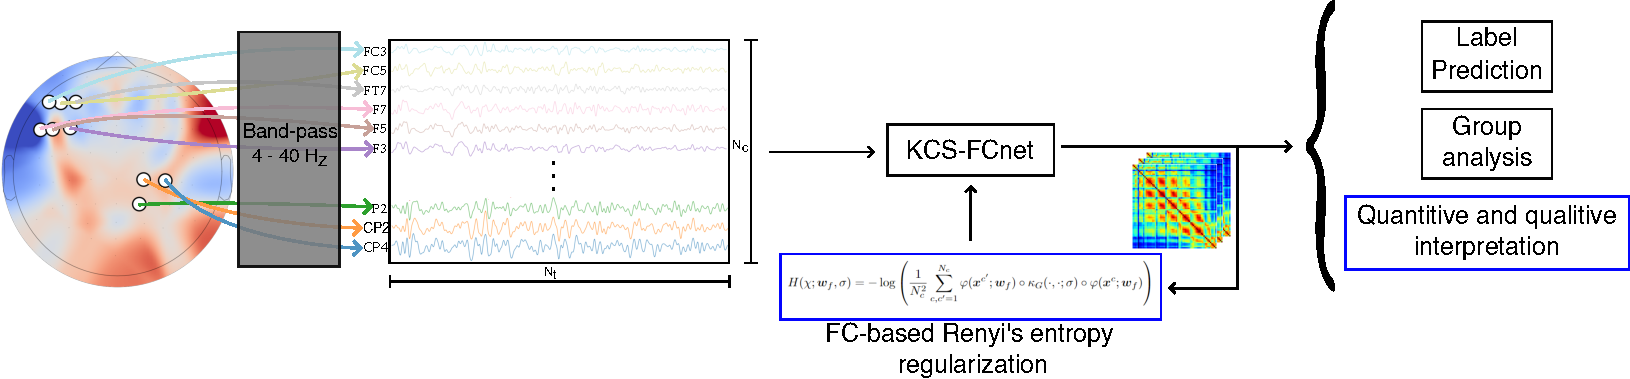
\includegraphics[scale=0.6]{Figures/outline_and_contributions/contribution3.pdf}
    \caption{Illustration of the proposed Interpretable Regularized Kernel Cross-Spectral Functional Connectivity Network (IRKCS-FCnet) model, with both qualitative and quantitative strategies for improved MI-BCI model explainability \label{fig:contribution3}}
\end{figure}


\section{Cross-Information Potential Regularization}

Let the set $\{\ve{X}^c \in \Real^{N_t} \}_{c=1}^{N_c}$ be i.i.d realizations drawn from the random variable $\chi$ with density function $\zeta(\chi)$. We can estimate the density function using the Parzen density estimation strategy as follow.

\begin{equation}
    \hat{\zeta}(\chi) = \frac{1}{N_c} \sum_{c=1}^{N_c} \kappa(\chi,x^c ; \sigma)
\end{equation}

Since the cross-information potential is a special case of the definite kernel $\kappa(\cdot,\cdot ; \sigma)$ and it is related to the Renyi's entropy $\alpha=2$ by a monotonic function as show in Equation~\eqref{eq:renyi_ent}. We can maximize either the Renyi's entropy or the cross-information potential.

\begin{equation}\label{eq:renyi_ent}
\begin{aligned}
    H_2(\chi) &= - \log \left( \int_{\chi} \hat{\zeta}(\chi)^2 \right) d\zeta \\
              &= - \log \left( \frac{1}{N_{c}^{2}} \sum_{c,c'=1}^{N_c} \kappa ( \ve{x}^{c} , \ve{x}^{c'} ) \right)
\end{aligned}
\end{equation}

This concept can be extended to the function composition proposed in \cref{chapter_2} Equation~\eqref{eq:CSf} as follows.

\begin{equation}
    \hat{\zeta}(\chi) = \frac{1}{N_c} \sum_{c=1}^{N_c}  {\kappa_{x}}(\chi,\cdot ; \sigma) \circ \varphi(\ve{x}^c; \ve{w}_f), 
\end{equation}
Where $\circ$ stands for function composition, $\varphi(\cdot; \mat{w}_f)$ is a 1-D convolutional layer that can be used to automatically extract frequency patterns ruled by the weight vector $\ve{w}_f\in \Real^{\Delta_t}$, with $\Delta_t<N_t$. Thus, the Renyi's entropy can be calculated as follow.

\changes{
\begin{equation}
  H(\chi; \mathbf{w}_f, \sigma) = - \log \left( \frac{1}{N_c^2} \sum_{c,c'=1}^{N_c} \kappa_{x}(\cdot, \cdot;\sigma) \circ\left (\varphi(x^{c'};w_f), \varphi(x^{c};w_f)\right ) \right) 
\end{equation}
}

Note that the maximal potential information is obtained when each sample provides a unique information about the Parzen estimation of the density function. Therefore, maximizing the cross-information potential will induce the diagonal $\mathbf{K}$ matrix. \changes{Since the main objective is to enhance the interpretability while maintaining the results obtained in \cref{chapter_2}, we include the $H(\chi; \mathbf{w}_f, \sigma)$ into the optimization problem as follows: 
\begin{equation}
  \Theta^{*} = \underset{\Theta}{\arg\,\min} \quad \promeddd{r}{\mathcal{L}(\ve{y}_r,\hat{\ve{y}}_r|\Theta) - H(\tilde{\mat{P}_r}; \mathbf{w}_f, \sigma); \forall r\in\{1,2,\dots,R\}},
\end{equation}
where $\tilde{\mat{P}}_r$ is the average functional connectivity measure calculated in Equation~\eqref{eq:lastlayerFC} and $\hat{\ve{y}}$ is the class probability vector obtained in Equation~\eqref{eq:output}. Here, the objective is akin to the information bottleneck principle, where we aim to maximize the cross-information potential while maintaining the accuracy obtained in \cref{chapter_2}. In this context, the cross-information potential serves as a regularization technique on the typical cross-entropy optimization problem.
}



\section{Experimental Set-Up}


\begin{itemize}

    \item[--] \textbf{Raw EEG Preprocessing:} The preprocessing stage starts with the loading of subject recordings using a \changes{custom database loader} module~(\url{https://github.com/UN-GCPDS/python-gcpds.databases}. Proceeding with the presumption that 2.5s windows are stationary, a Fourier method is applied to downsample each signal from 512 Hz to 128 Hz, as provided by the SciPy library with its signal resample function~\url{https://docs.scipy.org/doc/scipy/reference/generated/scipy.signal.resample.html}). Each time series trial is filtered within the $[4-40]$ Hz range using a fifth-order Butterworth bandpass filter. Subsequently, we construct an array of time-based records, utilizing 2.5s windows and a $50\%$ overlap, starting from 0s and ending at 7s. This enables us to analyze windows that contain no MI information, partial MI information, and solely MI information sequentially. It's important to note that the cue onset happens 2s post the start of the recording; this preprocessing tries to mirror the one in \cite{lawhern2018eegnet}. The filter $[4-40]$ Hz aimed at probing five distinct brain rhythms encompassing theta, alpha, and three beta waves \cite{ABHANG201651}. Where theta waves $[4-8]$ Hz, typically observed in the hippocampus and various cortical structures, are theorized to signify an ``online state'' and are linked with sensorimotor and mnemonic functionalities. On the contrary, alpha-band activity $[8-13]$ Hz is suppressed by sensory stimulation and movements, potentially acting as a marker for higher motor control functions given its modulation by attention, working memory, and mental tasks. The preprocessing also incorporates three beta wave types: ``beta one'' or low beta waves $[12-15]$ Hz typically correlate with focused and introverted focus; ``beta two'' or mid-range beta waves $[15-20]$ Hz are associated with augmented energy, anxiety, and performance; ``beta three'' or high beta waves $[18-40]$ Hz are indicative of considerable stress, anxiety, paranoia, high energy, and high arousal.

    \item[--] \textbf{Training:} Post-preprocessing, we are left with five datasets, each encapsulating 2.5s EEG information, all characterized by the same label set. Each dataset is individually trained as per the subsequent steps: Firstly, trials from each subject's data are split based on a standard $5$-fold $80$-$20$ scheme. In other words, the data is shuffled, and $80\%$ of it is utilized for training (forming the training set), withholding the remaining $20\%$ to validate the trained models (forming the testing set). This sequence is repeated five times in total. Subsequently, the plain model is trained with one of the training sets, searching for the hyperparameter $N_f$ within the set $\{2,3,4\}$ and $\Delta_t$ within the set $\{50,25\}$. It's important to note that the kernel length scale set corresponds with the new sampling frequency \cite{lawhern2018eegnet}. \changes{The ADAM algorithm \cite{kingma2014adam} is employed to tune the model parameters with a learning rate of $0.1$}. To locate the optimal combination of hyperparameters for our model, the GridSearchCV class from SKlearn is utilized. Given the need for performance comparison, we compute the accuracy, Cohen's kappa, and the area under the ROC curve to assess performance between models~\cite{warrens2015five,geron2022hands}. Following the conclusion of this procedure, the best performance metrics and hyperparameters are saved. For the sake of comparison, the optimal hyperparameters secured from the plain trained model are loaded onto the regularized version. The splitting and training steps are replicated similarly, except only for the new hyperparameter that modifies the regularization weight $\Upsilon$ on the cost function, and it is explored within the set $\{0,0.2,0.5,0.7,1,5,10\}$. Here, we aspire to compare the performance of the regularized version using the same hyperparameters over the identical time window. The underlying hypothesis is that the regularized version performs at least equivalently, or superior, to the plain version. We also aim to gain insights into how regularization impacts the connectivity matrix. Concluding the training process, we have ten models for each subject: five corresponding to the plain model and five to its regularized version.

    \item[--] \textbf{Model Level Analysis:} By leveraging the benchmark EEGnet model, we contrast the performances of both plain and regularized models. Subjects are sorted based on their respective EEGnet accuracy score. In addition, we examine the accuracy of each of the five windows mentioned above, analyzing how performance attenuates when the provision of MI information is constrained. For instance, we start when subjects see a blank screen, followed by moments entirely consumed by MI tasks, and finally reach situations where subjects behold a blank screen immediately after executing an MI task. In this final instance, the brain might continue engaging with the MI task for several seconds more. This comparative analysis promises to provide insights into the effects of varying MI information availability on model performance. 

    \item[--] \textbf{Group Level Analysis:} Focusing on the window demonstrating the highest performance, we use the k-means clustering algorithm~\cite{geron2022hands} to cluster the accuracy scores of each subject. Setting $k$ to three, we create a model categorizing subjects' performance based on their results in the EEGnet model~\cite{lawhern2018eegnet}. This separates the subjects into three distinct performance groups: best (G I), intermediate (G II), and worst (G III) performers. Applying this trained k-means model, we then cluster the data from the plain and regularized models. The aim here is to identify shifts in group assignments between the baseline performance and the results from plain and regularized models. To further our analysis, we calculate Renyi's entropy for each identified group, where higher Renyi's entropy implies a sparser connectivity matrix and higher cross-information potential. 
    \begin{itemize}
        \item[--] \textbf{Post-hoc interpretability:} We also examine the quantitative differences between the plain and regularized model versions, specifically looking at average and random feature drops. Using a paired t-test, we validate that dropping relevant features impacts accuracy differently than dropping random features. This involves creating scenarios where $5\%$, $10\%$, $15\%$, $20\%$, and $25\%$ of features are dropped based on relevance and randomly. The impact on accuracy in each scenario is then compared to the performance when all features are considered. By concatenating these calculated accuracy drop values and running a paired t-test, we verify their statistical difference. Given that our regularized version is designed to extract more relevant features, we expect to observe higher accuracy drop values with each drop percentage increase compared with its plain version.

        \item[--] \textbf{Intrinsic interpretability:} We also took the weights of the last layer to understand which channels were the most important. To do so, we calculated the values of the average weights for each group. Then, we summed up the absolute values for each branch class's average weights, sorted them, and took the top ten channels. Next, we represented them in a topoplot-like illustration. The hypothesis is that the best group will have all or most of the most important channels near the sensorimotor cortex area. While the noise affects the subjects with lower accuracy performance, the most important channels can be found in different areas. Furthermore, we extracted the Power Spectral Density (PSD) with the Welch method of the CNN layer output to analyze how the temporal and spectral filters modify the signals. This was done for each subject and then averaged by groups. Here, we are specifically interested in exploring the alpha wave, particularly the mu rhythm, oscillating between $8$ and \changes{$13 Hz$}. Activation of this rhythm, found primarily in motor-related brain areas, is hypothesized to be activated in the highest performing group \cite{hobson2017interpretation, llanos2013mu}. For other groups, a more widespread activation should be seen. In addition, the average of the last branch class weights is used to show the overall importance of each channel. This is shown by a 2D scalp representation, which aids in seeing which brain areas are the most important for each group. Here, we hypothesize that the sensorimotor areas are the most important for the best groups, while more areas are included as we approach the worst-performing group.
    \end{itemize}

    \item[--] \textbf{Individual Subject Analysis:} For a deep-dive into each group's characteristics, we select the subjects closest to their respective group's centroid for analysis. We initially calculate the PSD using the Welch method over cross and direct-label class normalized activation maps with the modified LayerCAM, which return one map per filter. The primary goal is to examine the relative importance of each filter coupled with the frequencies they extracted. We hypothesize that information will mostly be retained by the direct class, where each filter ideally should contribute equally towards the classification objective.
\end{itemize}  


\section{Results and Discussion}

\subsection{Model Level Analysis}

\cref{fig:acc_windows} shows the comparison of performance between different windows, each containing various amounts of MI information. The first window has no MI information, the second one contains half of the MI task, the third 0.5 seconds after the cue along with the complete span of MI information, the fourth comprises half MI and half post MI, and finally, the last window exclusively captures post-MI information.



\begin{figure}[h!]
  \centering
  \resizebox{\linewidth}{!}{% This file was created with tikzplotlib v0.10.1.
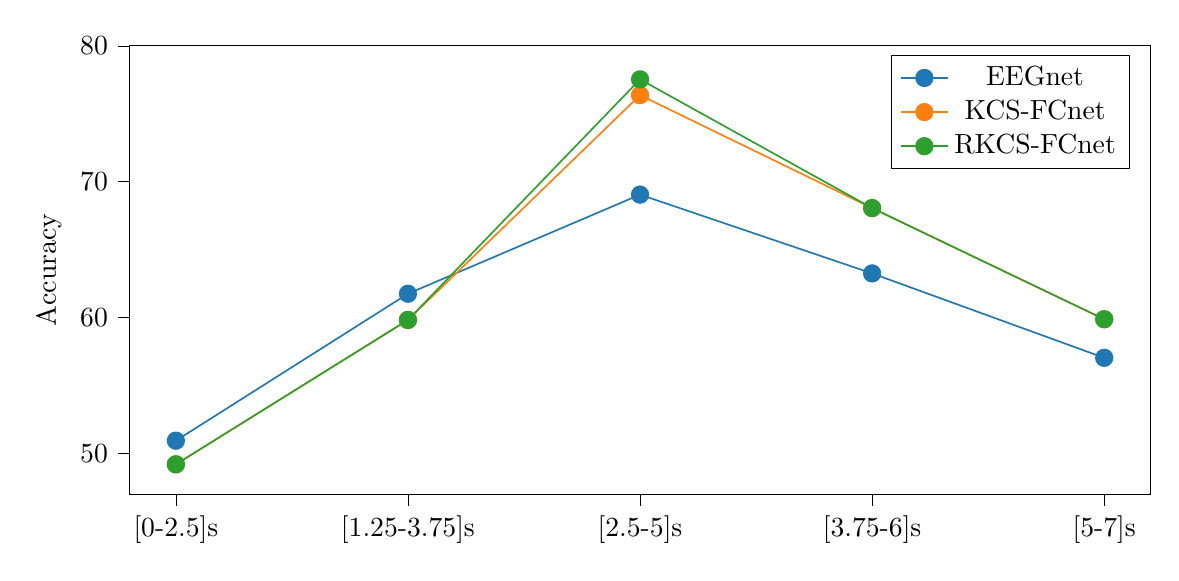
\begin{tikzpicture}

\definecolor{darkgray176}{RGB}{176,176,176}
\definecolor{darkorange25512714}{RGB}{255,127,14}
\definecolor{forestgreen4416044}{RGB}{44,160,44}
\definecolor{steelblue31119180}{RGB}{31,119,180}

\begin{axis}[
tick align=outside,
tick pos=left,
width=1.2\textwidth,
height=0.6\textwidth,
x grid style={darkgray176},
xmin=-0.2, xmax=4.2,
xtick style={color=black},
xtick={0,1,2,3,4},
xticklabels={[0-2.5]s,[1.25-3.75]s,[2.5-5]s,[3.75-6]s,[5-7]s},
y grid style={darkgray176},
ylabel={Accuracy},
ymin=47, ymax=80,
ytick style={color=black}
]
\addplot [semithick, steelblue31119180, mark=*, mark size=3, mark options={solid}]
table {%
0 50.9343747143037
1 61.7496471455741
2 69.0458206616888
3 63.2484703143283
4 57.0335169465879
};
\addplot [semithick, darkorange25512714, mark=*, mark size=3, mark options={solid}]
table {%
0 49.1931422217751
1 59.8215643889214
2 76.3688821731479
3 68.0560775205583
4 59.8733358252709
};
\addplot [semithick, forestgreen4416044, mark=*, mark size=3, mark options={solid}]
table {%
0 49.1931422217751
1 59.8215643889214
2 77.5303862995242
3 68.0560775205583
4 59.8733358252709
};
\addlegendentry{EEGnet}
\addlegendentry{KCS-FCnet}
\addlegendentry{RKCS-FCnet}

\end{axis}

\end{tikzpicture}
}
  \caption{Performance comparison across EEGnet (${\lineplot{steelblue31119180}}$), KCS-FCnet (${\lineplot{darkorange25512714}}$), and RKCS-FCnet (${\lineplot{forestgreen4416044}}$) models at different time windows.}\label{fig:acc_windows}
\end{figure}

The figure reveals three distinct patterns. Firstly, all three models exhibit an overall accuracy lower than 65\% when operating with none or insufficient MI information. Also, it is important to highlight that for these initial two windows, the EEGnet model outperforms the others, demonstrating a higher accuracy score. This can be attributed to the fact that FC-based models compare full-time windows to derive the connectivity matrix, making them more susceptible to windows conveying information from varied cognitive tasks. Moreover, as EEGnet continues to add more convolution layers, the impact of non-relevant time segments becomes minor. Secondly, all models hit their peak accuracy in the $[2.5-5]s$ window. Within this window, we observe roughly equivalent average accuracy between the two FC-based models, but there is a significant difference from the EEGnet. Thirdly, the phase of windows carrying post-MI information still shows greater accuracy performance than the first two windows, even though it contains post-task information. There could be residual information, as the brain may continue engaging with the task. Interestingly, a noticeable difference in accuracy score for the FC-based models is seen only in the best-performing window. This could occur because the regularization works optimally when the whole matrix represents the time segment holding the MI class under analysis. Henceforth, our focus will be on the best-performing window $[2.5-5]s$ for deeper analysis.

\begin{figure}[h!]
  \centering
  \resizebox{\linewidth}{!}{% This file was created with tikzplotlib v0.10.1.
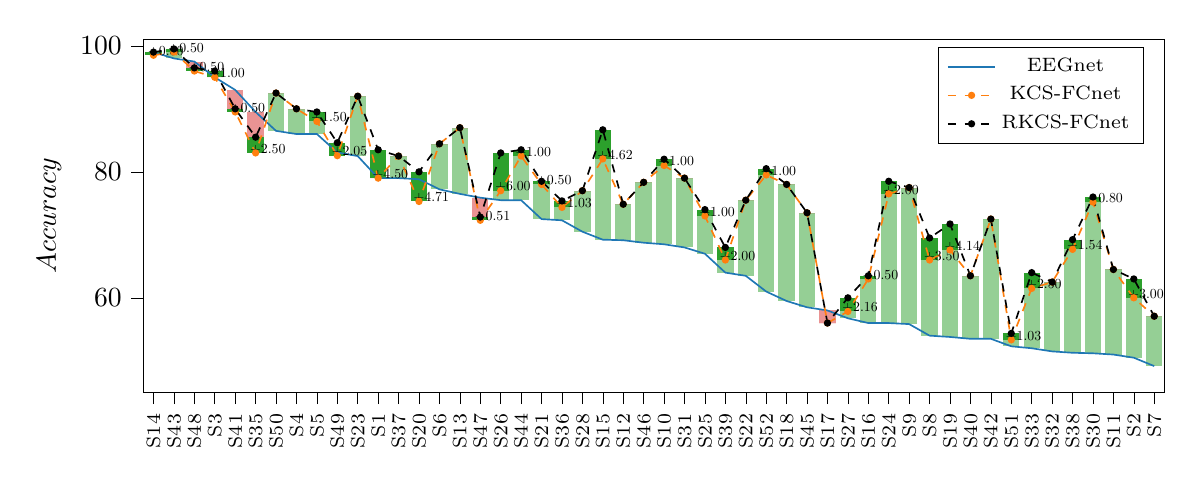
\begin{tikzpicture}

\definecolor{crimson2143940}{RGB}{214,39,40}
\definecolor{darkgray176}{RGB}{176,176,176}
\definecolor{darkorange25512714}{RGB}{255,127,14}
\definecolor{forestgreen4416044}{RGB}{44,160,44}
\definecolor{steelblue31119180}{RGB}{31,119,180}

\begin{axis}[
tick align=outside,
tick pos=left,
width=1.2\textwidth,
height=.5\textwidth,
x grid style={darkgray176},
xmin=-0.5, xmax=49.5,
xtick style={color=black},
xtick={0,1,2,3,4,5,6,7,8,9,10,11,12,13,14,15,16,17,18,19,20,21,22,23,24,25,26,27,28,29,30,31,32,33,34,35,36,37,38,39,40,41,42,43,44,45,46,47,48,49},
xticklabel style={rotate=90.0,anchor=east, font=\scriptsize},
xticklabels={
  S14,
  S43,
  S48,
  S3,
  S41,
  S35,
  S50,
  S4,
  S5,
  S49,
  S23,
  S1,
  S37,
  S20,
  S6,
  S13,
  S47,
  S26,
  S44,
  S21,
  S36,
  S28,
  S15,
  S12,
  S46,
  S10,
  S31,
  S25,
  S39,
  S22,
  S52,
  S18,
  S45,
  S17,
  S27,
  S16,
  S24,
  S9,
  S8,
  S19,
  S40,
  S42,
  S51,
  S33,
  S32,
  S38,
  S30,
  S11,
  S2,
  S7,
},
y grid style={darkgray176},
ylabel={$Accuracy$},
ymin=45, ymax=101,
ytick style={color=black},
legend style={font=\scriptsize}
]
\draw[draw=none,fill=crimson2143940,fill opacity=0.5] (axis cs:-0.4,99) rectangle (axis cs:0.4,98.5);
\draw[draw=none,fill=forestgreen4416044,fill opacity=0.5] (axis cs:0.6,98) rectangle (axis cs:1.4,99);
\draw[draw=none,fill=crimson2143940,fill opacity=0.5] (axis cs:1.6,97.5) rectangle (axis cs:2.4,96);
\draw[draw=none,fill=crimson2143940,fill opacity=0.5] (axis cs:2.6,95) rectangle (axis cs:3.4,95);
\draw[draw=none,fill=crimson2143940,fill opacity=0.5] (axis cs:3.6,93) rectangle (axis cs:4.4,89.5);
\draw[draw=none,fill=crimson2143940,fill opacity=0.5] (axis cs:4.6,89.5) rectangle (axis cs:5.4,83);
\draw[draw=none,fill=forestgreen4416044,fill opacity=0.5] (axis cs:5.6,86.5) rectangle (axis cs:6.4,92.5);
\draw[draw=none,fill=forestgreen4416044,fill opacity=0.5] (axis cs:6.6,86) rectangle (axis cs:7.4,90);
\draw[draw=none,fill=forestgreen4416044,fill opacity=0.5] (axis cs:7.6,86) rectangle (axis cs:8.4,88);
\draw[draw=none,fill=crimson2143940,fill opacity=0.5] (axis cs:8.6,83.0769230769231) rectangle (axis cs:9.4,82.5641025641026);
\draw[draw=none,fill=forestgreen4416044,fill opacity=0.5] (axis cs:9.6,82.5) rectangle (axis cs:10.4,92);
\draw[draw=none,fill=crimson2143940,fill opacity=0.5] (axis cs:10.6,79) rectangle (axis cs:11.4,79);
\draw[draw=none,fill=forestgreen4416044,fill opacity=0.5] (axis cs:11.6,79) rectangle (axis cs:12.4,82.5);
\draw[draw=none,fill=crimson2143940,fill opacity=0.5] (axis cs:12.6,78.8235294117647) rectangle (axis cs:13.4,75.2941176470588);
\draw[draw=none,fill=forestgreen4416044,fill opacity=0.5] (axis cs:13.6,77.2222222222222) rectangle (axis cs:14.4,84.4444444444444);
\draw[draw=none,fill=forestgreen4416044,fill opacity=0.5] (axis cs:14.6,76.5) rectangle (axis cs:15.4,87);
\draw[draw=none,fill=crimson2143940,fill opacity=0.5] (axis cs:15.6,75.8974358974359) rectangle (axis cs:16.4,72.3076923076923);
\draw[draw=none,fill=forestgreen4416044,fill opacity=0.5] (axis cs:16.6,75.5) rectangle (axis cs:17.4,77);
\draw[draw=none,fill=forestgreen4416044,fill opacity=0.5] (axis cs:17.6,75.5) rectangle (axis cs:18.4,82.5);
\draw[draw=none,fill=forestgreen4416044,fill opacity=0.5] (axis cs:18.6,72.5) rectangle (axis cs:19.4,78);
\draw[draw=none,fill=forestgreen4416044,fill opacity=0.5] (axis cs:19.6,72.3076923076923) rectangle (axis cs:20.4,74.3589743589744);
\draw[draw=none,fill=forestgreen4416044,fill opacity=0.5] (axis cs:20.6,70.5) rectangle (axis cs:21.4,77);
\draw[draw=none,fill=forestgreen4416044,fill opacity=0.5] (axis cs:21.6,69.2307692307692) rectangle (axis cs:22.4,82.051282051282);
\draw[draw=none,fill=forestgreen4416044,fill opacity=0.5] (axis cs:22.6,69.1428571428572) rectangle (axis cs:23.4,74.8571428571429);
\draw[draw=none,fill=forestgreen4416044,fill opacity=0.5] (axis cs:23.6,68.75) rectangle (axis cs:24.4,78.3333333333333);
\draw[draw=none,fill=forestgreen4416044,fill opacity=0.5] (axis cs:24.6,68.5) rectangle (axis cs:25.4,81);
\draw[draw=none,fill=forestgreen4416044,fill opacity=0.5] (axis cs:25.6,68) rectangle (axis cs:26.4,79);
\draw[draw=none,fill=forestgreen4416044,fill opacity=0.5] (axis cs:26.6,67) rectangle (axis cs:27.4,73);
\draw[draw=none,fill=forestgreen4416044,fill opacity=0.5] (axis cs:27.6,64) rectangle (axis cs:28.4,66);
\draw[draw=none,fill=forestgreen4416044,fill opacity=0.5] (axis cs:28.6,63.5) rectangle (axis cs:29.4,75.5);
\draw[draw=none,fill=forestgreen4416044,fill opacity=0.5] (axis cs:29.6,61) rectangle (axis cs:30.4,79.5);
\draw[draw=none,fill=forestgreen4416044,fill opacity=0.5] (axis cs:30.6,59.5) rectangle (axis cs:31.4,78);
\draw[draw=none,fill=forestgreen4416044,fill opacity=0.5] (axis cs:31.6,58.5) rectangle (axis cs:32.4,73.5);
\draw[draw=none,fill=crimson2143940,fill opacity=0.5] (axis cs:32.6,58) rectangle (axis cs:33.4,56);
\draw[draw=none,fill=forestgreen4416044,fill opacity=0.5] (axis cs:33.6,56.7567567567568) rectangle (axis cs:34.4,57.8378378378379);
\draw[draw=none,fill=forestgreen4416044,fill opacity=0.5] (axis cs:34.6,56) rectangle (axis cs:35.4,63);
\draw[draw=none,fill=forestgreen4416044,fill opacity=0.5] (axis cs:35.6,56) rectangle (axis cs:36.4,76.5);
\draw[draw=none,fill=forestgreen4416044,fill opacity=0.5] (axis cs:36.6,55.8333333333333) rectangle (axis cs:37.4,77.5);
\draw[draw=none,fill=forestgreen4416044,fill opacity=0.5] (axis cs:37.6,54) rectangle (axis cs:38.4,66);
\draw[draw=none,fill=forestgreen4416044,fill opacity=0.5] (axis cs:38.6,53.7931034482759) rectangle (axis cs:39.4,67.5862068965517);
\draw[draw=none,fill=forestgreen4416044,fill opacity=0.5] (axis cs:39.6,53.5) rectangle (axis cs:40.4,63.5);
\draw[draw=none,fill=forestgreen4416044,fill opacity=0.5] (axis cs:40.6,53.5) rectangle (axis cs:41.4,72.5);
\draw[draw=none,fill=forestgreen4416044,fill opacity=0.5] (axis cs:41.6,52.3076923076923) rectangle (axis cs:42.4,53.3333333333333);
\draw[draw=none,fill=forestgreen4416044,fill opacity=0.5] (axis cs:42.6,52) rectangle (axis cs:43.4,61.5);
\draw[draw=none,fill=forestgreen4416044,fill opacity=0.5] (axis cs:43.6,51.5) rectangle (axis cs:44.4,62.5);
\draw[draw=none,fill=forestgreen4416044,fill opacity=0.5] (axis cs:44.6,51.2820512820513) rectangle (axis cs:45.4,67.6923076923077);
\draw[draw=none,fill=forestgreen4416044,fill opacity=0.5] (axis cs:45.6,51.2) rectangle (axis cs:46.4,75.2);
\draw[draw=none,fill=forestgreen4416044,fill opacity=0.5] (axis cs:46.6,51) rectangle (axis cs:47.4,64.5);
\draw[draw=none,fill=forestgreen4416044,fill opacity=0.5] (axis cs:47.6,50.5) rectangle (axis cs:48.4,60);
\draw[draw=none,fill=forestgreen4416044,fill opacity=0.5] (axis cs:48.6,49.1666666666667) rectangle (axis cs:49.4,57.0833333333333);
\draw[draw=none,fill=forestgreen4416044] (axis cs:-0.4,98.5) rectangle (axis cs:0.4,99);
\draw[draw=none,fill=forestgreen4416044] (axis cs:0.6,99) rectangle (axis cs:1.4,99.5);
\draw[draw=none,fill=forestgreen4416044] (axis cs:1.6,96) rectangle (axis cs:2.4,96.5);
\draw[draw=none,fill=forestgreen4416044] (axis cs:2.6,95) rectangle (axis cs:3.4,96);
\draw[draw=none,fill=forestgreen4416044] (axis cs:3.6,89.5) rectangle (axis cs:4.4,90);
\draw[draw=none,fill=forestgreen4416044] (axis cs:4.6,83) rectangle (axis cs:5.4,85.5);
\draw[draw=none,fill=crimson2143940] (axis cs:5.6,92.5) rectangle (axis cs:6.4,92.5);
\draw[draw=none,fill=crimson2143940] (axis cs:6.6,90) rectangle (axis cs:7.4,90);
\draw[draw=none,fill=forestgreen4416044] (axis cs:7.6,88) rectangle (axis cs:8.4,89.5);
\draw[draw=none,fill=forestgreen4416044] (axis cs:8.6,82.5641025641026) rectangle (axis cs:9.4,84.6153846153846);
\draw[draw=none,fill=crimson2143940] (axis cs:9.6,92) rectangle (axis cs:10.4,92);
\draw[draw=none,fill=forestgreen4416044] (axis cs:10.6,79) rectangle (axis cs:11.4,83.5);
\draw[draw=none,fill=crimson2143940] (axis cs:11.6,82.5) rectangle (axis cs:12.4,82.5);
\draw[draw=none,fill=forestgreen4416044] (axis cs:12.6,75.2941176470588) rectangle (axis cs:13.4,80);
\draw[draw=none,fill=crimson2143940] (axis cs:13.6,84.4444444444444) rectangle (axis cs:14.4,84.4444444444444);
\draw[draw=none,fill=crimson2143940] (axis cs:14.6,87) rectangle (axis cs:15.4,87);
\draw[draw=none,fill=forestgreen4416044] (axis cs:15.6,72.3076923076923) rectangle (axis cs:16.4,72.8205128205128);
\draw[draw=none,fill=forestgreen4416044] (axis cs:16.6,77) rectangle (axis cs:17.4,83);
\draw[draw=none,fill=forestgreen4416044] (axis cs:17.6,82.5) rectangle (axis cs:18.4,83.5);
\draw[draw=none,fill=forestgreen4416044] (axis cs:18.6,78) rectangle (axis cs:19.4,78.5);
\draw[draw=none,fill=forestgreen4416044] (axis cs:19.6,74.3589743589744) rectangle (axis cs:20.4,75.3846153846154);
\draw[draw=none,fill=crimson2143940] (axis cs:20.6,77) rectangle (axis cs:21.4,77);
\draw[draw=none,fill=forestgreen4416044] (axis cs:21.6,82.051282051282) rectangle (axis cs:22.4,86.6666666666667);
\draw[draw=none,fill=crimson2143940] (axis cs:22.6,74.8571428571429) rectangle (axis cs:23.4,74.8571428571429);
\draw[draw=none,fill=crimson2143940] (axis cs:23.6,78.3333333333333) rectangle (axis cs:24.4,78.3333333333333);
\draw[draw=none,fill=forestgreen4416044] (axis cs:24.6,81) rectangle (axis cs:25.4,82);
\draw[draw=none,fill=crimson2143940] (axis cs:25.6,79) rectangle (axis cs:26.4,79);
\draw[draw=none,fill=forestgreen4416044] (axis cs:26.6,73) rectangle (axis cs:27.4,74);
\draw[draw=none,fill=forestgreen4416044] (axis cs:27.6,66) rectangle (axis cs:28.4,68);
\draw[draw=none,fill=crimson2143940] (axis cs:28.6,75.5) rectangle (axis cs:29.4,75.5);
\draw[draw=none,fill=forestgreen4416044] (axis cs:29.6,79.5) rectangle (axis cs:30.4,80.5);
\draw[draw=none,fill=crimson2143940] (axis cs:30.6,78) rectangle (axis cs:31.4,78);
\draw[draw=none,fill=crimson2143940] (axis cs:31.6,73.5) rectangle (axis cs:32.4,73.5);
\draw[draw=none,fill=crimson2143940] (axis cs:32.6,56) rectangle (axis cs:33.4,56);
\draw[draw=none,fill=forestgreen4416044] (axis cs:33.6,57.8378378378378) rectangle (axis cs:34.4,60);
\draw[draw=none,fill=forestgreen4416044] (axis cs:34.6,63) rectangle (axis cs:35.4,63.5);
\draw[draw=none,fill=forestgreen4416044] (axis cs:35.6,76.5) rectangle (axis cs:36.4,78.5);
\draw[draw=none,fill=crimson2143940] (axis cs:36.6,77.5) rectangle (axis cs:37.4,77.5);
\draw[draw=none,fill=forestgreen4416044] (axis cs:37.6,66) rectangle (axis cs:38.4,69.5);
\draw[draw=none,fill=forestgreen4416044] (axis cs:38.6,67.5862068965517) rectangle (axis cs:39.4,71.7241379310345);
\draw[draw=none,fill=crimson2143940] (axis cs:39.6,63.5) rectangle (axis cs:40.4,63.5);
\draw[draw=none,fill=forestgreen4416044] (axis cs:40.6,72.5) rectangle (axis cs:41.4,72.5);
\draw[draw=none,fill=forestgreen4416044] (axis cs:41.6,53.3333333333333) rectangle (axis cs:42.4,54.3589743589744);
\draw[draw=none,fill=forestgreen4416044] (axis cs:42.6,61.5) rectangle (axis cs:43.4,64);
\draw[draw=none,fill=crimson2143940] (axis cs:43.6,62.5) rectangle (axis cs:44.4,62.5);
\draw[draw=none,fill=forestgreen4416044] (axis cs:44.6,67.6923076923077) rectangle (axis cs:45.4,69.2307692307692);
\draw[draw=none,fill=forestgreen4416044] (axis cs:45.6,75.2) rectangle (axis cs:46.4,76);
\draw[draw=none,fill=crimson2143940] (axis cs:46.6,64.5) rectangle (axis cs:47.4,64.5);
\draw[draw=none,fill=forestgreen4416044] (axis cs:47.6,60) rectangle (axis cs:48.4,63);
\draw[draw=none,fill=crimson2143940] (axis cs:48.6,57.0833333333333) rectangle (axis cs:49.4,57.0833333333333);
\addplot [semithick, steelblue31119180]
table {%
0 99
1 98
2 97.5
3 95
4 93
5 89.5
6 86.5
7 86
8 86
9 83.0769230769231
10 82.5
11 79
12 79
13 78.8235294117647
14 77.2222222222222
15 76.5
16 75.8974358974359
17 75.5
18 75.5
19 72.5
20 72.3076923076923
21 70.5
22 69.2307692307692
23 69.1428571428572
24 68.75
25 68.5
26 68
27 67
28 64
29 63.5
30 61
31 59.5
32 58.5
33 58
34 56.7567567567568
35 56
36 56
37 55.8333333333333
38 54
39 53.7931034482759
40 53.5
41 53.5
42 52.3076923076923
43 52
44 51.5
45 51.2820512820513
46 51.2
47 51
48 50.5
49 49.1666666666667
};
\addplot [semithick, darkorange25512714, mark=*, mark size=1, mark options={solid}, dashed]
table {%
0 98.5
1 99
2 96
3 95
4 89.5
5 83
6 92.5
7 90
8 88
9 82.5641025641026
10 92
11 79
12 82.5
13 75.2941176470588
14 84.4444444444444
15 87
16 72.3076923076923
17 77
18 82.5
19 78
20 74.3589743589744
21 77
22 82.051282051282
23 74.8571428571429
24 78.3333333333333
25 81
26 79
27 73
28 66
29 75.5
30 79.5
31 78
32 73.5
33 56
34 57.8378378378378
35 63
36 76.5
37 77.5
38 66
39 67.5862068965517
40 63.5
41 72.5
42 53.3333333333333
43 61.5
44 62.5
45 67.6923076923077
46 75.2
47 64.5
48 60
49 57.0833333333333
};
\addplot [semithick, black, mark=*, mark size=1, mark options={solid}, dashed]
table {%
0 99
1 99.5
2 96.5
3 96
4 90
5 85.5
6 92.5
7 90
8 89.5
9 84.6153846153846
10 92
11 83.5
12 82.5
13 80
14 84.4444444444444
15 87
16 72.8205128205128
17 83
18 83.5
19 78.5
20 75.3846153846154
21 77
22 86.6666666666667
23 74.8571428571429
24 78.3333333333333
25 82
26 79
27 74
28 68
29 75.5
30 80.5
31 78
32 73.5
33 56
34 60
35 63.5
36 78.5
37 77.5
38 69.5
39 71.7241379310345
40 63.5
41 72.5
42 54.3589743589744
43 64
44 62.5
45 69.2307692307692
46 76
47 64.5
48 63
49 57.0833333333333
};
\addlegendentry{EEGnet}
\addlegendentry{KCS-FCnet}
\addlegendentry{RKCS-FCnet}
\draw (axis cs:0.6,97.5) node[
  scale=0.5,
  anchor=south,
  text=black,
  rotate=0.0
]{+0.50};
\draw (axis cs:1.6,98) node[
  scale=0.5,
  anchor=south,
  text=black,
  rotate=0.0
]{+0.50};
\draw (axis cs:2.6,95) node[
  scale=0.5,
  anchor=south,
  text=black,
  rotate=0.0
]{+0.50};
\draw (axis cs:3.6,94) node[
  scale=0.5,
  anchor=south,
  text=black,
  rotate=0.0
]{+1.00};
\draw (axis cs:4.6,88.5) node[
  scale=0.5,
  anchor=south,
  text=black,
  rotate=0.0
]{+0.50};
\draw (axis cs:5.6,82) node[
  scale=0.5,
  anchor=south,
  text=black,
  rotate=0.0
]{+2.50};
\draw (axis cs:8.6,87) node[
  scale=0.5,
  anchor=south,
  text=black,
  rotate=0.0
]{+1.50};
\draw (axis cs:9.6,81.5641025641026) node[
  scale=0.5,
  anchor=south,
  text=black,
  rotate=0.0
]{+2.05};
\draw (axis cs:11.6,78) node[
  scale=0.5,
  anchor=south,
  text=black,
  rotate=0.0
]{+4.50};
\draw (axis cs:13.6,74.2941176470588) node[
  scale=0.5,
  anchor=south,
  text=black,
  rotate=0.0
]{+4.71};
\draw (axis cs:16.6,71.3076923076923) node[
  scale=0.5,
  anchor=south,
  text=black,
  rotate=0.0
]{+0.51};
\draw (axis cs:17.6,76) node[
  scale=0.5,
  anchor=south,
  text=black,
  rotate=0.0
]{+6.00};
\draw (axis cs:18.6,81.5) node[
  scale=0.5,
  anchor=south,
  text=black,
  rotate=0.0
]{+1.00};
\draw (axis cs:19.6,77) node[
  scale=0.5,
  anchor=south,
  text=black,
  rotate=0.0
]{+0.50};
\draw (axis cs:20.6,73.3589743589744) node[
  scale=0.5,
  anchor=south,
  text=black,
  rotate=0.0
]{+1.03};
\draw (axis cs:22.6,81.051282051282) node[
  scale=0.5,
  anchor=south,
  text=black,
  rotate=0.0
]{+4.62};
\draw (axis cs:25.6,80) node[
  scale=0.5,
  anchor=south,
  text=black,
  rotate=0.0
]{+1.00};
\draw (axis cs:27.6,72) node[
  scale=0.5,
  anchor=south,
  text=black,
  rotate=0.0
]{+1.00};
\draw (axis cs:28.6,65) node[
  scale=0.5,
  anchor=south,
  text=black,
  rotate=0.0
]{+2.00};
\draw (axis cs:30.6,78.5) node[
  scale=0.5,
  anchor=south,
  text=black,
  rotate=0.0
]{+1.00};
\draw (axis cs:34.6,56.8378378378378) node[
  scale=0.5,
  anchor=south,
  text=black,
  rotate=0.0
]{+2.16};
\draw (axis cs:35.6,62) node[
  scale=0.5,
  anchor=south,
  text=black,
  rotate=0.0
]{+0.50};
\draw (axis cs:36.6,75.5) node[
  scale=0.5,
  anchor=south,
  text=black,
  rotate=0.0
]{+2.00};
\draw (axis cs:38.6,65) node[
  scale=0.5,
  anchor=south,
  text=black,
  rotate=0.0
]{+3.50};
\draw (axis cs:39.6,66.5862068965517) node[
  scale=0.5,
  anchor=south,
  text=black,
  rotate=0.0
]{+4.14};
\draw (axis cs:42.6,52.3333333333333) node[
  scale=0.5,
  anchor=south,
  text=black,
  rotate=0.0
]{+1.03};
\draw (axis cs:43.6,60.5) node[
  scale=0.5,
  anchor=south,
  text=black,
  rotate=0.0
]{+2.50};
\draw (axis cs:45.6,66.6923076923077) node[
  scale=0.5,
  anchor=south,
  text=black,
  rotate=0.0
]{+1.54};
\draw (axis cs:46.6,74.2) node[
  scale=0.5,
  anchor=south,
  text=black,
  rotate=0.0
]{+0.80};
\draw (axis cs:48.6,59) node[
  scale=0.5,
  anchor=south,
  text=black,
  rotate=0.0
]{+3.00};
\end{axis}

\end{tikzpicture}}
  \caption{Comparison of subject-specific average accuracy across EEGnet, KCS-FCnet, and RKCS-FCnet models. Subjects are arranged in descending order based on the accuracy of the EEGnet model. The color-coded bars illustrate performance shifts, with dark green(\legend{forestgreen4416044}) indicating an increase in accuracy on the RKCS-FCnet over KCS-FCnet, light green(\legend{forestgreen4416044!50}) indicating an increase in accuracy on KCS-FCnet over EEGnet, and while red \legend{crimson2143940!50} indicates an accuracy reduction.}\label{fig:accuracy_sbj_comp}
\end{figure}



\Cref{fig:accuracy_sbj_comp} illustrates a comparative analysis of the accuracy rates achieved by the EEGnet, KCS-FCnet, and RKCS-FCnet models over the best performing window $[0.5-2.5]s$. It provides a visual representation of the average accuracy for individual subjects. Subjects have been ordered based on the accuracy performance of EEGnet, depicted as a blue line, and the dotted orange and black lines, respectively denote the KCS-FCnet and RKCS-FCnet models. Changes in accuracy are represented by color coding, where green indicates an increase in accuracy, whereas red signifies a decrease. Additionally, the differential accuracy between the plain and regularized versions is presented with solid green bars and numerical values for comparative evaluation, highlighting how much advancement the regularized version has achieved over its plain counterpart. For instance, it can be seen in subject 26, with a notable increase of six percentile points. Overall, both the KCS-FCnet and RKCS-FCnet models outperform the benchmark model, with only a few exceptions where the accuracy drops. It's interesting to note that the regularized version consistently performs at least as well as, or better than, the plain version, with an accuracy boost of more than four percentage points observed for subjects 1, 20, 26, and 15. It is worth noting that increases in accuracy were not significant in subjects already achieving more than $80\%$ accuracy, suggesting strong predictive power offered by either approach for those subjects. However, subjects falling below $80\%$ FC-based methods demonstrated the most marked improvements, particularly under the $70\%$ threshold, where the nature of FC effectively prevents noisy connections. Lastly, the overall comparison illustrates that subject 17 yields identical performance across all three models.

\subsection{Group Level Analysis}

\begin{figure}[!h]
  \centering
  \resizebox{\linewidth}{!}{% This file was created with tikzplotlib v0.10.1.
\begin{tikzpicture}

\definecolor{darkgray176}{RGB}{176,176,176}

\begin{axis}[
tick align=outside,
tick pos=left,
width=1\textwidth,
height=.5\textwidth,
x grid style={darkgray176},
xmin=-0.5, xmax=49.5,
xtick style={color=black},
xtick={0,1,2,3,4,5,6,7,8,9,10,11,12,13,14,15,16,17,18,19,20,21,22,23,24,25,26,27,28,29,30,31,32,33,34,35,36,37,38,39,40,41,42,43,44,45,46,47,48,49},
xticklabel style={rotate=90.0},
xticklabels={
  S20,
  S40,
  S38,
  S48,
  S8,
  S45,
  S11,
  S3,
  S41,
  S30,
  S15,
  S14,
  S27,
  S21,
  S35,
  S37,
  S32,
  S10,
  S42,
  S36,
  S17,
  S25,
  S6,
  S1,
  S33,
  S49,
  S22,
  S46,
  S24,
  S28,
  S7,
  S26,
  S51,
  S47,
  S31,
  S13,
  S12,
  S5,
  S4,
  S44,
  S9,
  S19,
  S2,
  S18,
  S52,
  S16,
  S39,
  S23,
  S43,
  S50
},
y dir=reverse,
y grid style={darkgray176},
ymin=-0.5, ymax=2.5,
ytick style={color=black},
ytick={0,1,2},
yticklabels={EEGnet,KCS-FCnet,RKCS-FCnet}
]
\addplot graphics [includegraphics cmd=\pgfimage,xmin=-0.5, xmax=49.5, ymin=2.5, ymax=-0.5] {Figures/Objective_3/semaforo.png};
\end{axis}

\end{tikzpicture}
}
  \caption{Group transitions for subjects across EEGnet, KCS-FCnet, and RKCS-FCnet models. The color representation, green, yellow, and red, correspondingly signifies the best, intermediate, and worst average accuracy performance. First row: Initial group allocation of subjects based on EEGnet model results. Second row: Subject group transitions resulting from implementing the KCS-FCnet model. Third row: Subject group shifts according to the outcomes of the RKCS-FCnet model.}\label{fig:belongcomp_obj3}
\end{figure}

\Cref{fig:belongcomp_obj3} illustrates the distribution of subjects across various performance groups for each approach. We use three colors (light green, light yellow, and light red) to differentiate the groups: best performance, intermediate performance, and worst performance, respectively. In the first row, we present the distribution of performance for the EEGnet model. This will serve as our benchmark for comparing distributions. The second row reveals a shift in group belonging when using the KCS-FCnet model. Specifically, five subjects from the intermediate group have moved to the best performing group, and twelve subjects advanced from the worst to the intermediate group. Note the significant concentration of subjects in the intermediate performance group. The same trend is observed in the third row, showcasing the group distribution for the RKCS-FCnet. Light-colored symbols mark subjects who remain in their initial group with same accuracy performance, while those with solid colors depict subjects with improved accuracy rates. For instance, subjects 14, 10, and 49 are promoted from the intermediate to the best group, while subjects 13 and 18 moved up from the worst to the intermediate group. It is worth noting that the regularized model maintains or enhances subject group standings and accuracy. For the RKCS-FCnet model only six subjects are left in the worst performance group. This marks an improvement compared to the eight subjects under the KCS-FCnet model and a significant advance from the twenty in the same group under our baseline EEGnet model. In fact, performance was found to be improved for 31 subjects as compared to the KCS-FCnet model. Thus, the incorporation of FC information offers notable advantages, especially in aiding the subjects from the worst performance group, more so when combined with Renyi's regularization.

\begin{table}
    \centering
    \caption{Comparison of accuracy performance across groups and models}
    \label{tab:acc_obj3}    
    \begin{tabular}{|c|c|c|c|}
        \hline
        Strategy & G I & G II  & G III \\
        \hline
        EEGnet & 90.55 $\pm$ 5.88 & 72.15 $\pm$ 4.87 & 54.27 $\pm$ 3.21 \\
        KCS-FCnet & 91.46 $\pm$ 5.31   &  77.85 $\pm$ 4.76 & 66.66 $\pm$ 7.88 \\
        IRKCS-FCnet & \textbf{92.28 $\pm$ 4.79}  & \textbf{79.26 $\pm$ 4.93}  & \textbf{67.77$\pm$ 7.83} \\
        \hline
    \end{tabular}
\end{table}

\Cref{tab:acc_obj3} provides a comparative perspective on the accuracy performance of three models (EEGnet, KCS-FCnet, IRKCS-FCnet)  across the three distinct groups, where bold numbers represent the highest group score. Each group varies based on performance—from the highest performing (Group I) to the lowest (Group III). Note that The regularized version (IRKCS-FCnet) reaches the highest accuracy scores. In Group I, the accuracy difference is marginal at about one percentage point between the EEGnet baseline and KCS-FCnet. Yet, the improvement becomes more marked with the IRKCS-FCnet, which outpaces the baseline by nearly two percentage points. Interestingly, the standard deviation for the regularized version also witnesses a decrease of more than one percentage point, suggesting enhanced consistency in performance for the regularized version. Group II exemplifies the most dramatic difference in accuracy, with an uplift from 72.15\% in EEGnet to almost 80\% in RKCS-FCnet. Despite the nearly constant standard deviation across all models in this group, the number of subjects included in this group increases significantly for the FC-based models compared to the baseline model, indicating greater stability. Finally, in Group III, the FC-based models perform similarly, outperforming the baseline model by over 12 percentage points. The most substantial difference between FC-based and baseline models is seen in this group; a possible explanation for this substantial improvement is that FC information plays a critical role in enhancing the model's performance, particularly for subjects with potentially noisier EEG recordings, as evident in \cref{fig:accuracy_sbj_comp}.


\begin{figure}[!h]
  \centering
  \resizebox{\linewidth}{!}{% This file was created with tikzplotlib v0.10.1.
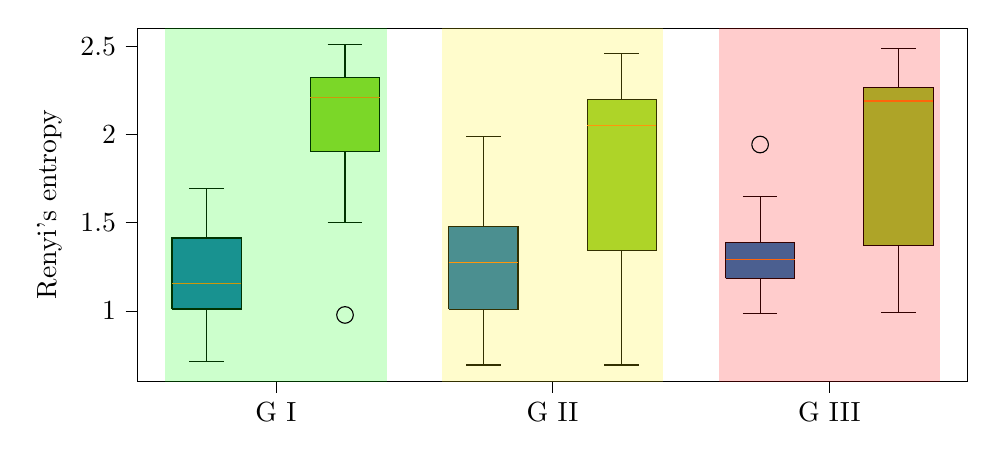
\begin{tikzpicture}

\definecolor{darkgray176}{RGB}{176,176,176}
\definecolor{darkorange25512714}{RGB}{255,127,14}

\definecolor{steelblue31119180}{RGB}{31,119,180}
\definecolor{yellowgreen}{RGB}{154, 205, 50}

\begin{axis}[
tick align=outside,
tick pos=left,
x grid style={darkgray176},
xmin=0.5, xmax=6.5,
width=\textwidth,
height=0.5\textwidth,
xtick style={color=black},
xtick={1.5,3.5,5.5},
xticklabels={G I,G II,G III},
y grid style={darkgray176},
ylabel={Renyi's entropy},
ymin=0.602331051230431, ymax=2.60267644226551,
ytick style={color=black}
]
\addplot [black, fill=steelblue31119180]
table {%
0.75 1.0111822783947
1.25 1.0111822783947
1.25 1.41367989778519
0.75 1.41367989778519
0.75 1.0111822783947
};
\addplot [black]
table {%
1 1.0111822783947
1 0.714407742023468
};
\addplot [black]
table {%
1 1.41367989778519
1 1.69561421871185
};
\addplot [black]
table {%
0.875 0.714407742023468
1.125 0.714407742023468
};
\addplot [black]
table {%
0.875 1.69561421871185
1.125 1.69561421871185
};
\addplot [black, fill=yellowgreen]
table {%
1.75 1.90198284387589
2.25 1.90198284387589
2.25 2.32088589668274
1.75 2.32088589668274
1.75 1.90198284387589
};
\addplot [black]
table {%
2 1.90198284387589
2 1.49933624267578
};
\addplot [black]
table {%
2 2.32088589668274
2 2.51175165176392
};
\addplot [black]
table {%
1.875 1.49933624267578
2.125 1.49933624267578
};
\addplot [black]
table {%
1.875 2.51175165176392
2.125 2.51175165176392
};
\addplot [black, mark=o, mark size=3, mark options={solid,fill opacity=0}, only marks]
table {%
2 0.977205276489258
};
\addplot [black, fill=steelblue31119180]
table {%
2.75 1.00999590754509
3.25 1.00999590754509
3.25 1.47894328832626
2.75 1.47894328832626
2.75 1.00999590754509
};
\addplot [black]
table {%
3 1.00999590754509
3 0.693255841732025
};
\addplot [black]
table {%
3 1.47894328832626
3 1.99005436897278
};
\addplot [black]
table {%
2.875 0.693255841732025
3.125 0.693255841732025
};
\addplot [black]
table {%
2.875 1.99005436897278
3.125 1.99005436897278
};
\addplot [black, fill=yellowgreen]
table {%
3.75 1.34344190359116
4.25 1.34344190359116
4.25 2.19900119304657
3.75 2.19900119304657
3.75 1.34344190359116
};
\addplot [black]
table {%
4 1.34344190359116
4 0.69325590133667
};
\addplot [black]
table {%
4 2.19900119304657
4 2.46135926246643
};
\addplot [black]
table {%
3.875 0.69325590133667
4.125 0.69325590133667
};
\addplot [black]
table {%
3.875 2.46135926246643
4.125 2.46135926246643
};
\addplot [black, fill=steelblue31119180]
table {%
4.75 1.18452069163322
5.25 1.18452069163322
5.25 1.38582560420036
4.75 1.38582560420036
4.75 1.18452069163322
};
\addplot [black]
table {%
5 1.18452069163322
5 0.987190246582031
};
\addplot [black]
table {%
5 1.38582560420036
5 1.65000188350677
};
\addplot [black]
table {%
4.875 0.987190246582031
5.125 0.987190246582031
};
\addplot [black]
table {%
4.875 1.65000188350677
5.125 1.65000188350677
};
\addplot [black, mark=o, mark size=3, mark options={solid,fill opacity=0}, only marks]
table {%
5 1.94329965114594
};
\addplot [black, fill=yellowgreen]
table {%
5.75 1.36978048086166
6.25 1.36978048086166
6.25 2.2656888961792
5.75 2.2656888961792
5.75 1.36978048086166
};
\addplot [black]
table {%
6 1.36978048086166
6 0.992337465286255
};
\addplot [black]
table {%
6 2.2656888961792
6 2.48897361755371
};
\addplot [black]
table {%
5.875 0.992337465286255
6.125 0.992337465286255
};
\addplot [black]
table {%
5.875 2.48897361755371
6.125 2.48897361755371
};
\addplot [darkorange25512714]
table {%
0.75 1.15490031242371
1.25 1.15490031242371
};
\addplot [darkorange25512714]
table {%
1.75 2.20872807502747
2.25 2.20872807502747
};
\addplot [darkorange25512714]
table {%
2.75 1.27640020847321
3.25 1.27640020847321
};
\addplot [darkorange25512714]
table {%
3.75 2.0507481098175
4.25 2.0507481098175
};
\addplot [darkorange25512714]
table {%
4.75 1.29070019721985
5.25 1.29070019721985
};
\addplot [darkorange25512714]
table {%
5.75 2.19007635116577
6.25 2.19007635116577
};
\path [draw=green, opacity=0.2, line width=80pt]
(axis cs:1.5,0.1)
--(axis cs:1.5,3);

\path [draw=yellow, opacity=0.2, line width=80pt]
(axis cs:3.5,0.1)
--(axis cs:3.5,3);

\path [draw=red, opacity=0.2, line width=80pt]
(axis cs:5.5,0.1)
--(axis cs:5.5,3);
\end{axis}

\end{tikzpicture}
}
  \caption{Box and whisker plot comparing Renyi's entropy across groups for KCS-FCnet  (blue boxplots) and RKCS-FCnet (green boxplots) models. The background codes the group membership (best, intermediate, and worst performance
clusters)}
  \label{fig:renyi_obj3}
\end{figure}


As demonstrated in \cref{fig:renyi_obj3}, the regularized model consistently displays higher entropy values across all groups. Remember that within the cost function, along with cross-entropy, the pursuit of maximizing this specific value is prioritized. In this scenario, higher entropy values suggest that there is a greater focus on obtaining independent rows in the FC matrix, which in turn indicates the inclusion of less noisy connections. Group I shows the most significant difference. Except for one sample, all other samples exceed 1.5. This trend can be attributed to the fact that best-performing subjects might rely on fewer connections to achieve high accuracy, allowing for more effective regularization. A similar pattern is observed in Groups II and III, with increased entropy values seen in the regularized model's results in both cases. However, Group II showcases a wider spread of values. This could be explained by the larger number of subjects included in this group for both plain and regularized versions. The overlap seen in this box and whisker plot, becoming more extensive in the intermediate group, led us to perform a paired t-test. This statistical test helps ascertain whether the observed values can be considered as belonging to different sets, thus establishing the statistical difference between them. The assessed p-values for Groups I, II, and III were 0.00006, 0.00175, and 0.00005, respectively. All these p-values fall below the significance level of 0.05, with Groups I and III exhibiting exceptionally low p-values below 0.001. Consequently, this statistically significant variance reiterates that the values derived from the regularized model are distinctively different across all groups.

\subsubsection{Post-Hoc Interpretability}

\begin{table}[h!]
\centering
\caption{p-values comparing accuracy drop of KCS-FCnet and RKCS-FCnet models vs Random (* indicates p-value < 0.01)}\label{table:p_values}
\begin{tabular}{|c|c|c|}
\hline
\textbf{Group} & \textbf{KCS-FCnet vs. Random} & \textbf{RKCS-FCnet vs. Random} \\ \hline
\textbf{G I} & 0.00077* & 0.00230* \\
\textbf{G II} & 0.00368* & 0.00434* \\
\textbf{G III} & 0.00108* & 0.00074* \\ \hline
\end{tabular}
\end{table}

We quantified the average drop for both models to validate that IRKCS-FCnet is better at extracting relevant features than its plain version. Here, we progressively eliminate features from the most relevant and monitor the resultant decrease in accuracy performance. We introduced a random version for comparison to ensure valuable feature learning in both models. In this context, all features hold an equal likelihood of being dropped. As shown in \cref{table:p_values} the calculated p-values confirm that the drop in accuracy upon feature removal in both models is statistically different from the random drop across all performance groups (G I, G II, and G III).



\cellcolor{GII!80}
\cellcolor{GIII!80}


\begin{table}[h!]
\centering
\caption{Average accuracy drop across feature removal percentages for KCS-FCnet and RKCS-FCnet, with higher difference drops indicated by (\legend{GI!80}) for GI, (\legend{GII!80}) for GII, and (\legend{GIII!80}) for GIII.}\label{table:average_drop}
\begin{tabular}{|l|l|c|c|c|c|c|}
\hline
\textbf{Strategy} & \textbf{Group} & \textbf{25\%} & \textbf{20\%} & \textbf{15\%} & \textbf{10\%} & \textbf{5\%} \\ \hline
\multirow{3}{*}{\textbf{KCS-FCnet}} & \textbf{G I} & 40.51 & 37.93 & 35.97 & 30.25 & 17.12 \\
 & \textbf{G II} & 40.10 & 39.00 & 36.46 & \cellcolor{GII!80}28.60 & 17.72 \\
 & \textbf{G III} & 39.05 & 36.98 & 31.99 & 25.28 & 15.02 \\ \hline
\multirow{3}{*}{\textbf{RKCS-FCnet}} & \textbf{G I} &  44.80 & 39.21 &  37.79 &  30.55 & \cellcolor{GI!80} 22.46 \\
 & \textbf{G II} & 41.08 & 40.01 & 36.77 & 27.28 & 18.84 \\
 & \textbf{G III} & 39.65 & 37.30 & 33.12 & \cellcolor{GIII!80}27.10 & 16.80 \\ \hline
\end{tabular}
\end{table}


\Cref{table:average_drop} illustrates the decrease in accuracy as more important features are removed, with higher drop values indicating the removal of more critical features. Notably, in both models, groups that initially achieved higher accuracy scores suffer larger accuracy drops, especially when contrasted with other groups. This effect is particularly evident when only $5\%$ of the features are removed. Across all groups and every percentage of feature drops, barring one case for GII, the IRKCS-FCnet outperforms in terms of feature importance as it shows higher accuracy drops. Additionally, the most substantial differences are represented by (\legend{GI!80}) with a $5.34$ percentage points for GI, (\legend{GII!80}) with a $1.32$ percentage points gain for the plain model in the case of GII, and (\legend{GIII!80}) with a $1.82$ percentage points for GIII.

For instance, in Group I, the plain model suffers a drop of 17.12 accuracy points, whereas the regularized model experiences a more significant drop of 22.46 points, marking a difference of over 5 points. Similar but less pronounced differences are observed for Groups II and III. However, as we increase the feature removal amount to higher percentages, the discrepancy between the plain and regularized versions' drop values gradually diminishes. We can attribute this trend to the finite set of critical features. After their removal, eliminating additional features might not have the same level of impact. Moreover, Group I, as the top performing group, exhibits the largest drops until 15\% of removed features. It is worth noting that as we progress from removing 15\% to 25\% of features, all drop values seemingly plateau, approximating an accuracy drop of almost 40\%. Recalling that the MI task explored holds a binary classification, any dummy model would still be expected to achieve an average accuracy of about 50\%. Therefore, this observation of the models standing near to 40\% drop in accuracy as more features are removed underscores the relative significance of each feature in our models.


\subsubsection{Intrinsic Interpretability}

The top ten channels for each group can be seen in \cref{fig:topotoptenchans}. For Group I, the best-performing, we can see that most of the channels reside in the sensorimotor cortex (CP3, CP4, CP6), central sulcus (C1, C2, C3, C4, C6), and the motor cortex (FC2, FC4). As stated in various studies about individuals performing motor tasks, we can observe significant activation differences in contiguous structures such as the anterior and posterior areas of the central sulcus, motor cortex, and sensorimotor \cite{eichert2021morphological}. Moving on to Group II, the first notable difference is that the channels from the motor cortex are not among the top ten, with $60\%$ of the electrodes located in the motor-related brain area. The remaining $40\%$ are found on the parietal lobe (P1, P3, PO3, POz), a region primarily responsible for fine sensation related to sensory perception and integration. In this instance, this area may be activated due to the visuospatial navigation and reasoning when viewing the screen instructing to perform a specific Motor Imagery task. It is logical to infer visual stimuli interpretation is occurring since half of these channels are located in the parietal-occipital area \cite{phunruangsakao2023effects}. Lastly, in Group III, comprising the worst-performing individuals, we observe that only $30\%$ of the top ten channels are situated in the motor-related area (FC6, C3, CP3). The remaining $70\%$ consist of electrodes from temporal (TP7), parietal-occipital (PO7, POz, PO8), occipital (Oz, Iz - the most posterior occipital electrode), and prefrontal (Fp2) regions. The frontal and occipital lobes suggest that visual information remains influential in brain network organization. Specifically, the Fp2 channels may suggest the presence of high ocular artifacts \cite{han2023cepstral}.

\def \kerrwidth {0.3\linewidth}
\def \kerrg {0.3\linewidth}
\begin{figure}[h!]
\centering
\scalebox{0.95}[0.95]{
\begin{tabular}{ccc}
\centering
\textbf{G I} & \textbf{G II} & \textbf{G III} \\
{\resizebox{\kerrwidth}{!}{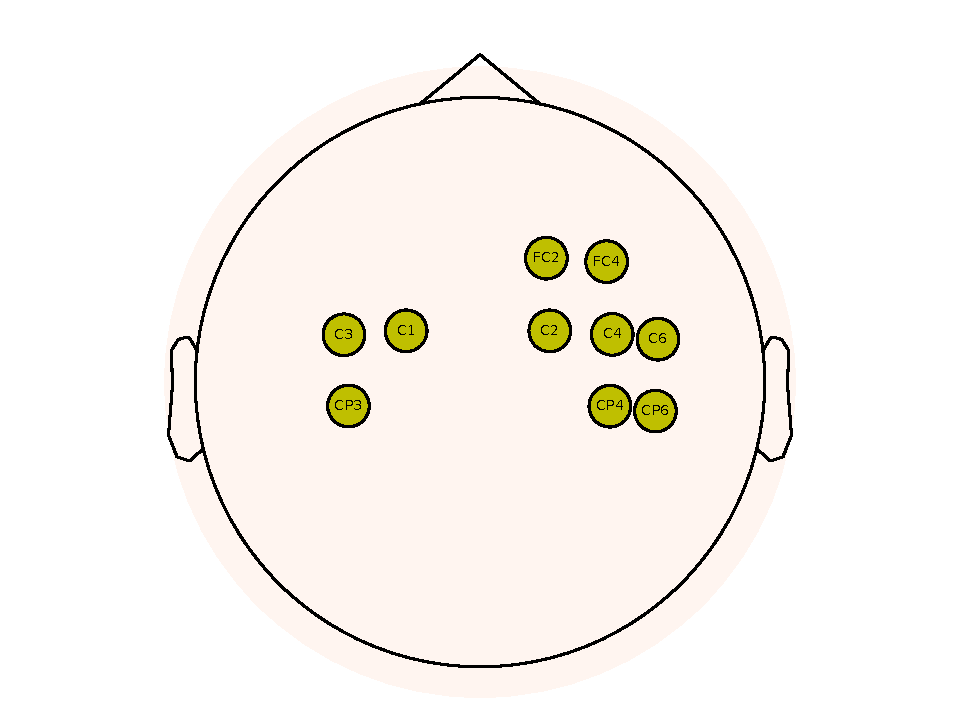
\includegraphics[trim=80 10 80 10, clip]{Figures/Objective_3/group_G I_top10_channels.pdf}}} & 
{\resizebox{\kerrwidth}{!}{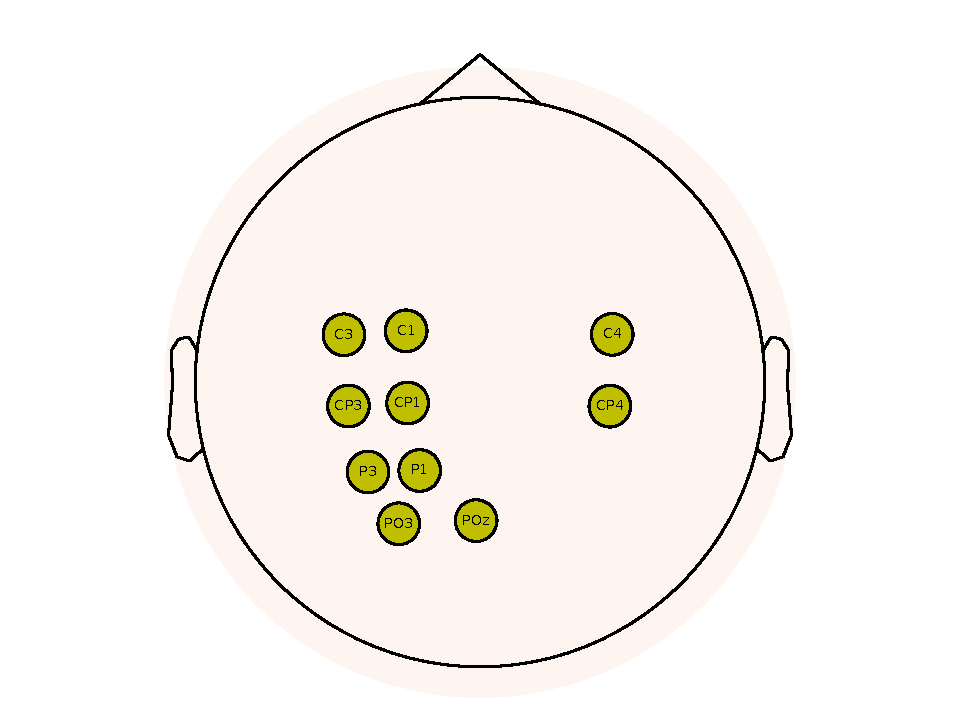
\includegraphics[trim=80 10 80 10, clip]{Figures/Objective_3/group_G II_top10_channels.pdf}}} & {\resizebox{\kerrwidth}{!}{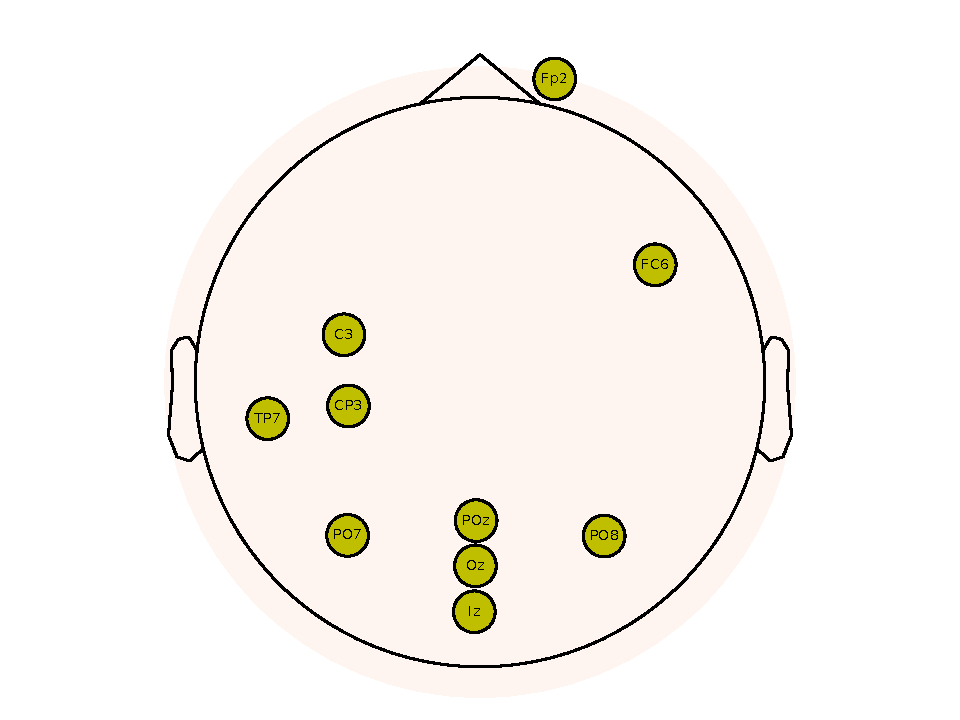
\includegraphics[trim=80 10 80 10, clip]{Figures/Objective_3/group_G III_top10_channels.pdf}}} \\
\end{tabular}
}
%\vspace{-42pt}
\caption{Visualization of the top ten channels in each group. The channels for Group I (left) are primarily concentrated in the sensorimotor cortex, central sulcus, and motor cortex. In Group II (middle), the majority of the channels are located in the motor-related brain area and parietal lobe, with visual stimuli interpretation inferred from the number of channels in the parietal-occipital area. For Group III (right), the top channels are predominantly located in non-motor-related areas, with a particular influence from visual information in the frontal and occipital lobes and possible high ocular artifacts suggested by the presence of Fp2 channels. \label{fig:topotoptenchans}}
\end{figure}

In order to gain a deeper understanding of the spectral filters produced by the CNN layer, \cref{fig:psdtopten} presents the average PSD for each group on the top ten channels, ranked in order of importance. In Group I, we observe a relatively stable spectrum, with the spectral power mainly concentrated between $10$ and \changes{$14 Hz$}, exhibiting higher spectral power centered around \changes{$12 Hz$}. This observation aligns with various studies noting that motor imagery-related tasks predominantly influence the Mu rhythm, oscillating between $8$ and \changes{$13 Hz$} \cite{al2021deep,hobson2017interpretation, llanos2013mu}. Group II demonstrates a similar pattern; however, the spectral power appears slightly skewed to the left. Nonetheless, it still falls within the range of the Mu oscillations associated with motor imagery in motor-related brain areas \cite{chen2021mu}. As for the last group, the pre-frontal Fp2 channel captures most of the spectral power, with significant influences from $\alpha$ and $\theta$ waves. With Oz and Fp2 emerging as the two most important channels and Fp2 commanding the majority of the spectral power, it can be inferred that a substantial amount of artifacts are introduced \cite{han2023cepstral}. These artifacts directly impact this group's task performance accuracy as we showed in \cref{tab:acc_obj3}.

\def \kerrwidth {0.7\linewidth}
\begin{figure}[h!]
\centering
\scalebox{0.95}[0.95]{
\begin{tabular}{cc}
\centering
{\rotatebox{90}{\hspace{12mm} \textbf{G I}}} &
{\resizebox{\kerrwidth}{!}{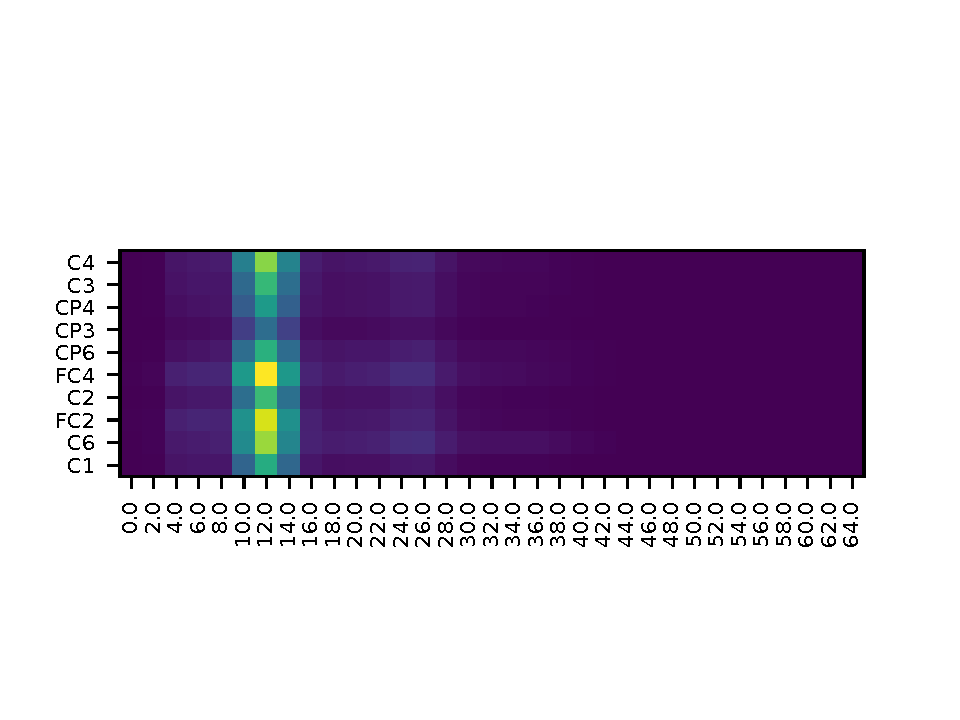
\includegraphics[trim=25 115 35 120, clip]{Figures/Objective_3/group_G I_top10_channels_PSD.pdf}}} \\

{\rotatebox{90}{\hspace{12mm} \textbf{G II}}} &
{\resizebox{\kerrwidth}{!}{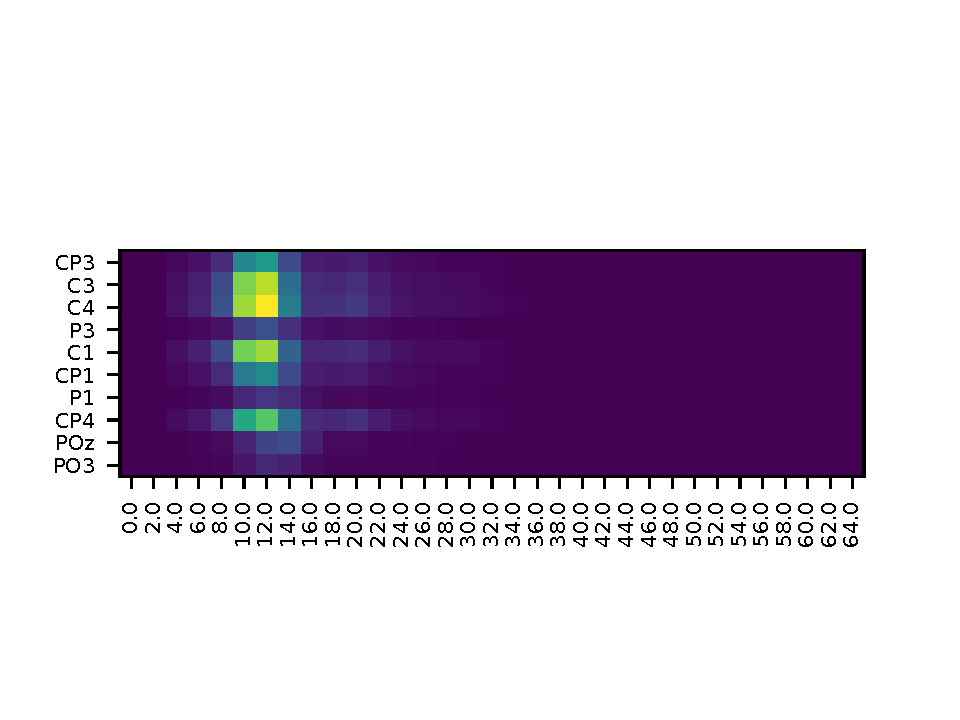
\includegraphics[trim=25 115 35 120, clip]{Figures/Objective_3/group_G II_top10_channels_PSD.pdf}}} \\

{\rotatebox{90}{\hspace{21mm} \textbf{G III}}} &
{\resizebox{\kerrwidth}{!}{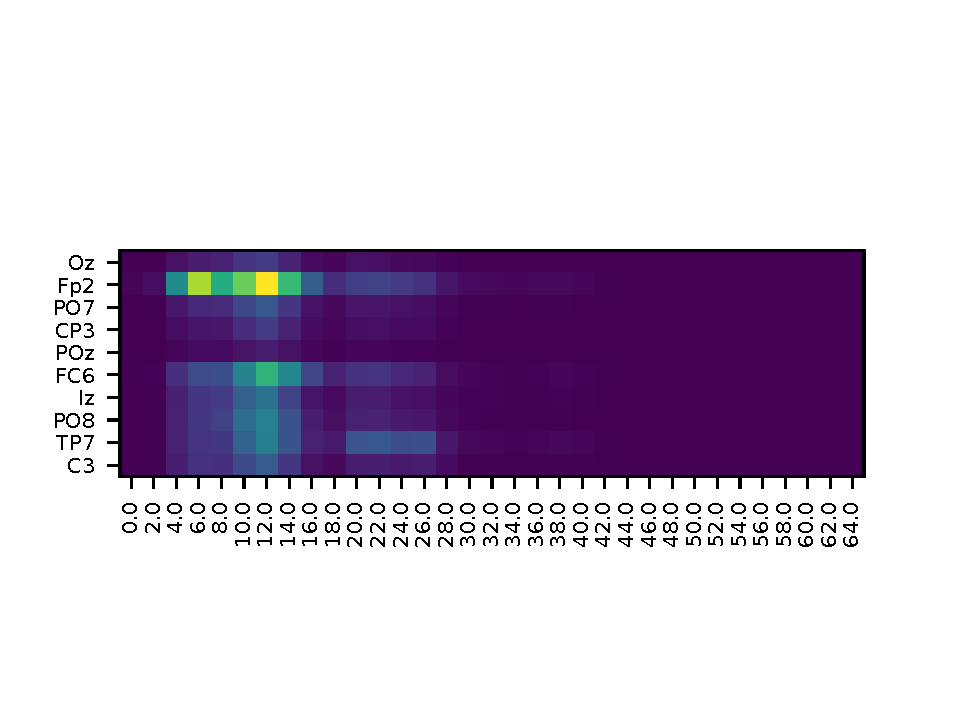
\includegraphics[trim=25 80 35 120, clip]{Figures/Objective_3/group_G III_top10_channels_PSD.pdf}}} \\
\end{tabular}
}
%\vspace{-42pt}
\caption{Illustration of the average PSD for each group plotted across the ten most important channels, categorized by importance from top to bottom. Relatively stable spectrum is visible within Group I (top), with predominant spectral power between $10$ and \changes{$14 Hz$}. Group II (middle) exhibits a similar pattern, with a slightly left-skewed power distribution, yet still within the range of Mu oscillations. On the contrary, Group III (bottom) displays an increase in spectral power at the pre-frontal Fp2 channel, significantly influenced by $\alpha$ and $\theta$ waves, indicating the introduction of substantial artifacts. \label{fig:psdtopten}}
\end{figure}


Figure \cref{fig:spatialint} offers a 2D illustration of scalp spatial relevance for each group and each class (Right and Left hand), enhancing our understanding of spatial interpretability. Clear activation is noted in the sensorimotor region for the first two groups, primarily for the left hand, with positive significance in the contralateral region and negative significance in the ipsilateral \cite{van2021frontal}. An inverse yet similar pattern is observed for the right hand. Group II displays a spread of importance that extends towards the parietal and occipital lobes yet retains a significant concentration around the sensorimotor cortex. For Group I, channels C3 and C4 are the most important, and channel CP3 is also highlighted for Group II. Group III shows an intriguing behavior with a faint contralateral arrangement for the left class and ipsilateral for the right. Nevertheless, numerous activations in non-motor-related external channels, like Fp2, Oz, PO8, and PO7, suggest a possibility of artifact interference \cite{collazos2023posthoc}. Intense activation observed in the occipital lobe could indicate the likely impact of substantial visual stimuli on processing motor-related information. These dispersed activations align with the modest accuracy level of around $68\%$ achieved in the IRKCS-FCnet. The proposed regularization method allows for efficient handling of artifacts and effective capture of crucial information around the motor-related brain area. However, in extreme situations, challenges persist. Even though an increase is observed in the accuracy level, nearing the $70\%$ threshold for BCI inefficiency, noise and artifacts continue to hinder the performance of the MI task \cite{vidaurre2021improving}.


\def \kerrwidth {0.3\linewidth}
\begin{figure}[h!]
\centering
\scalebox{0.95}[0.95]{
\begin{tabular}{ccccc}
\centering
& \textbf{G I} & \textbf{G II} & \textbf{G III} & \\
{\rotatebox{90}{\hspace{15mm} \textbf{Left class}}} & 
{\resizebox{\kerrwidth}{!}{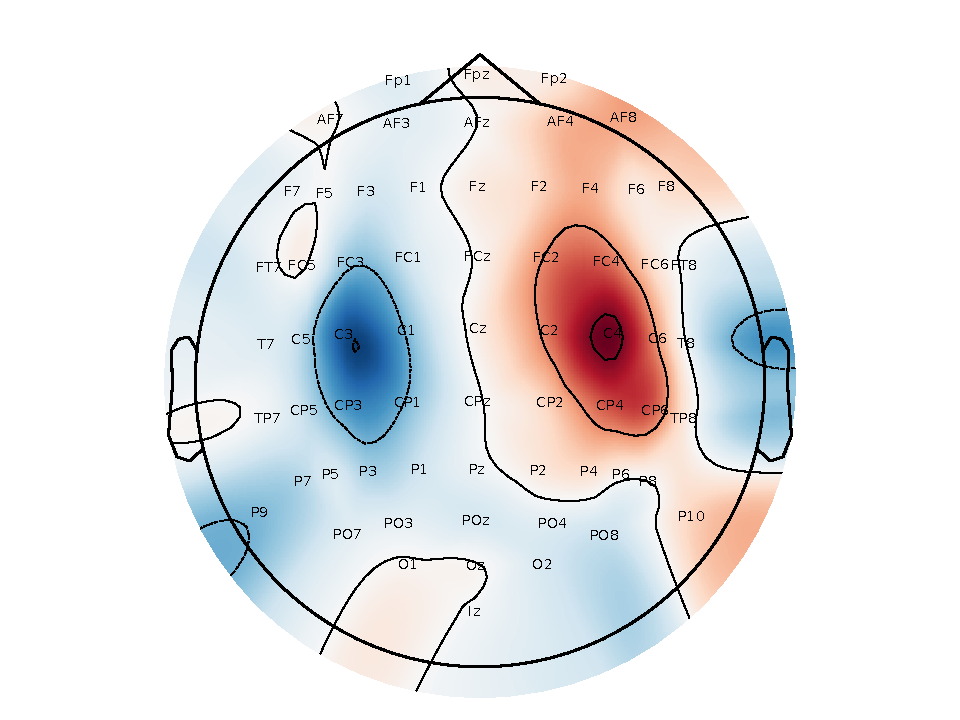
\includegraphics[trim=80 10 80 10, clip]{Figures/Objective_3/class_Left_group_G I_GFC_renyi.pdf}}} & 
{\resizebox{\kerrwidth}{!}{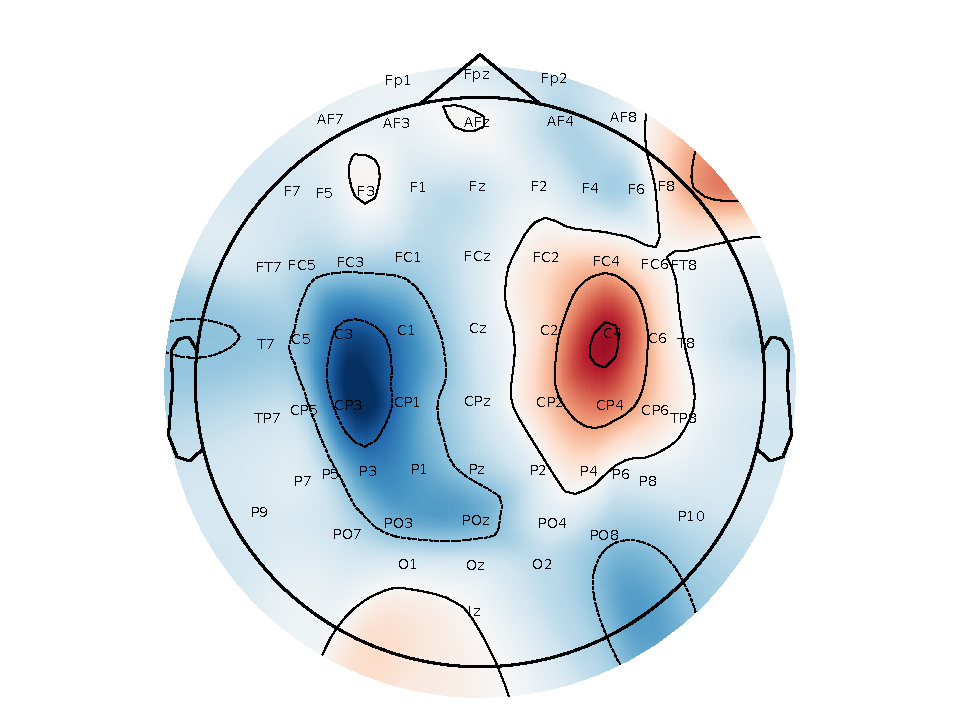
\includegraphics[trim=80 10 80 10, clip]{Figures/Objective_3/class_Left_group_G II_GFC_renyi.pdf}}} & {\resizebox{\kerrwidth}{!}{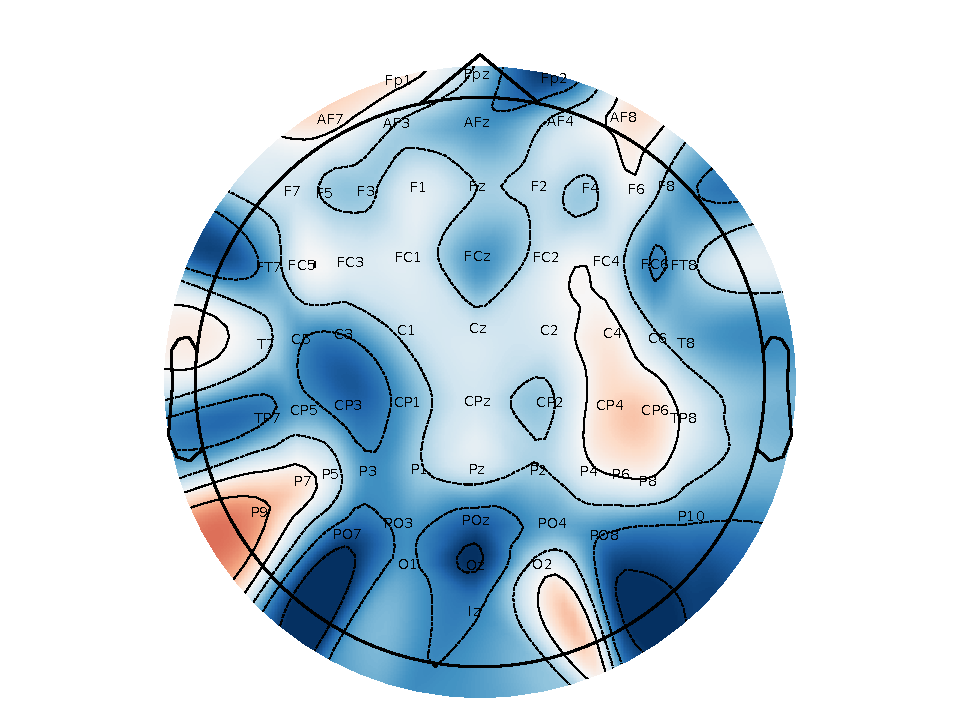
\includegraphics[trim=80 10 80 10, clip]{Figures/Objective_3/class_Left_group_G III_GFC_renyi.pdf}}} & \\
{\rotatebox{90}{\hspace{15mm} \textbf{Right class}}} & 
{\resizebox{\kerrwidth}{!}{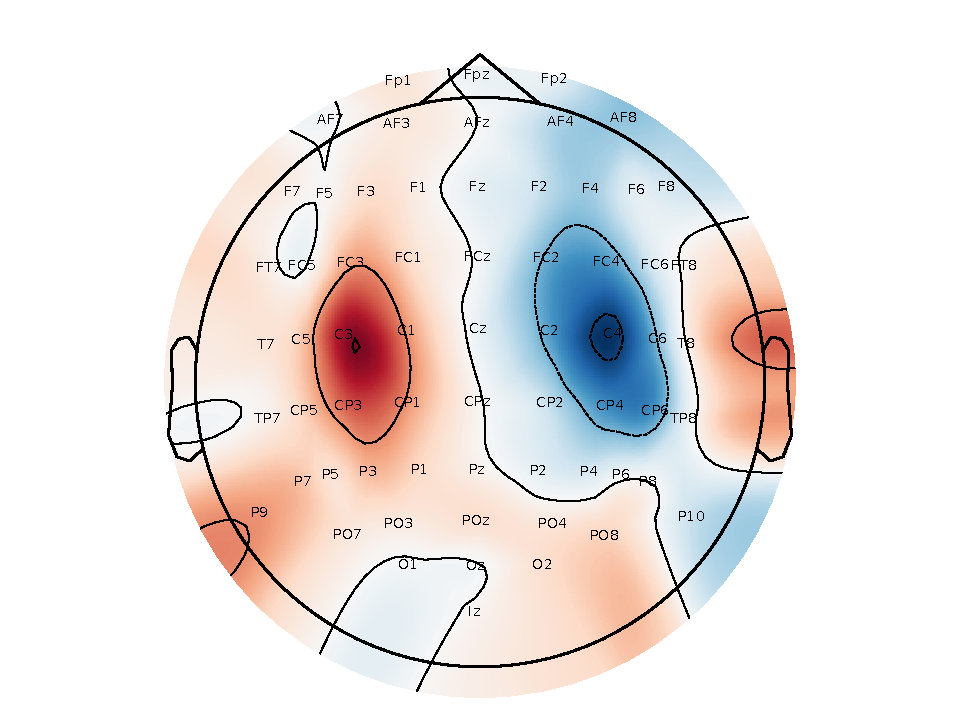
\includegraphics[trim=80 10 80 10, clip]{Figures/Objective_3/class_Right_group_G I_GFC_renyi.pdf}}} & 
{\resizebox{\kerrwidth}{!}{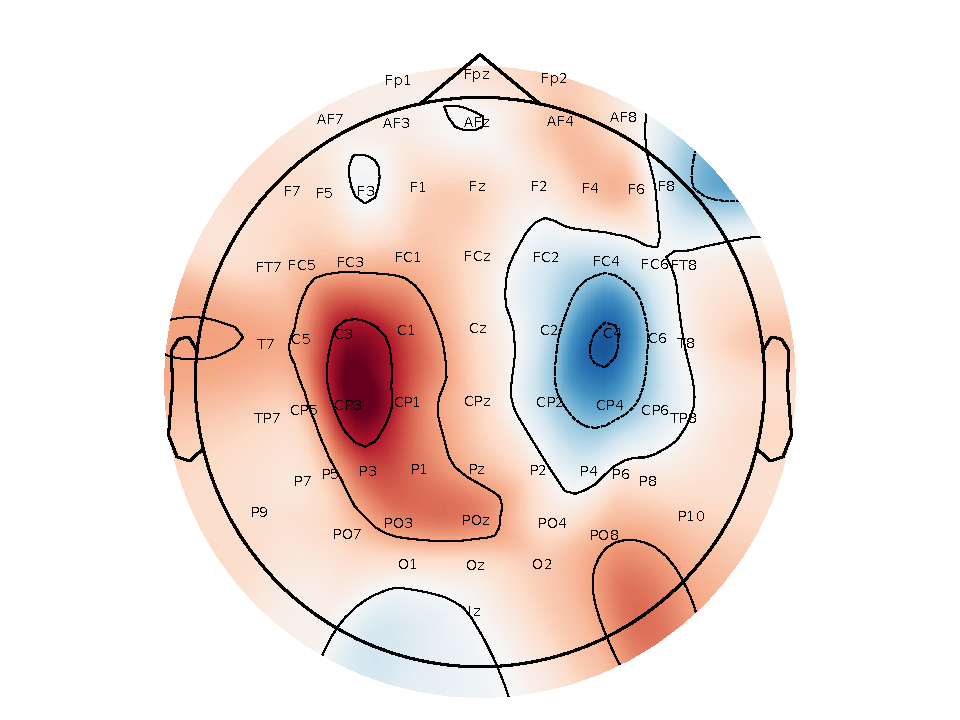
\includegraphics[trim=80 10 80 10, clip]{Figures/Objective_3/class_Right_group_G II_GFC_renyi.pdf}}} & {\resizebox{\kerrwidth}{!}{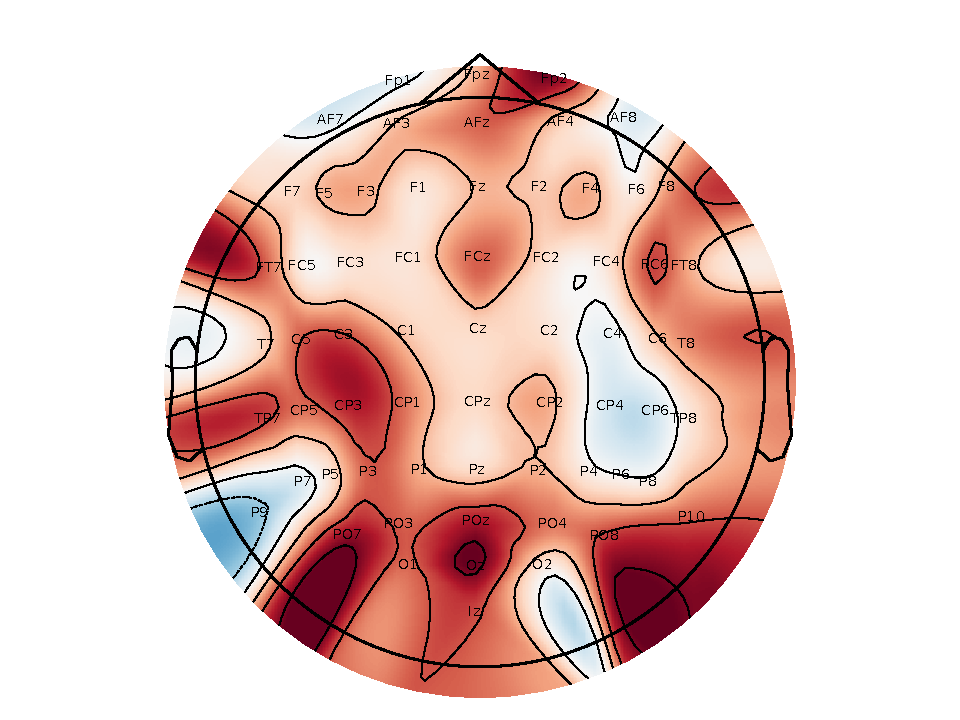
\includegraphics[trim=80 10 80 10, clip]{Figures/Objective_3/class_Right_group_G III_GFC_renyi.pdf}}} & \\
&\multicolumn{3}{c}{\resizebox{0.69\linewidth}{!}{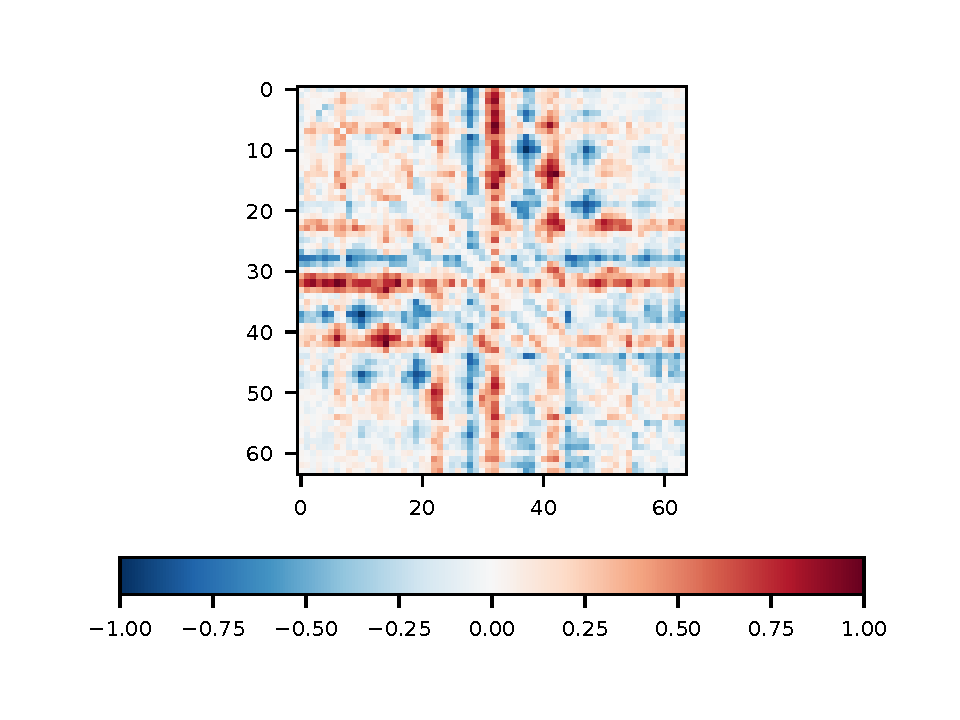
\includegraphics[trim=0 0 0 250, clip]{Figures/Objective_3/colorbar.pdf}}} \\
\end{tabular}
}
%\vspace{-42pt}
\caption{Spatial relevance for each group derived from the final layer of the IRKCS-FCnet model. The background represents the accumulated spatial relevance mapped to EEG channel positions. The first row represents the left class, while the second represents the right class. The columns are dedicated to each group: the left column for Group I, the middle column for Group II, and the right column for Group III. The figure visibly presents activation in sensorimotor regions across groups, potential artifact interferences, and alignment with the low accuracy level achieved in G III. \label{fig:spatialint}}
\end{figure}


\subsection{Individual Subject Analysis}

Figure \cref{fig:psd_ind_filt} displays individual subjects from Group I, Group II, and Group III, specifically subjects 4, 42, and 51, respectively. Across all cases, the cross-label importance is zero, thereby indicating no model misdirection towards the contrary class. While this is a positive aspect, the overall zero cross-label importance suggests potential overfitting in our model. For subject 4 of Group I, the direct label PSD shows that the $\alpha$ brain wave is primarily relevant for classifying the right-hand movement, as per the expectations for motor-related tasks. Interestingly, the left-hand movement assigns greater importance to higher frequency bands (around $20$ to \changes{$26 Hz$}) and no importance to motor-related frequencies. This pattern suggests a model bias towards the right class, indicating a potential increase in false positives (samples incorrectly classified as right-hand movement). In the case of subject 42 from Group II, who uses four filters, the critical frequencies seem somewhat dispersed yet primarily concentrated within the $10$ to \changes{$18 Hz$} range. Filters three and four, which highlight the motor-related frequencies, are most important. In contrast, the less critical filters extend across the entire available bandwidth. This scenario does not show any clear preferences between right and left classes. On the other hand, subject 51 from Group III, one of the individuals with the lowest performance, presents a distinct pattern. The most important frequencies, predominantly for the left-hand class, appear above motor-related frequencies, specifically around \changes{$28 Hz$}. The right-hand class does not exhibit comparable crucial filters or frequencies. Interestingly, for this class, most of the motor-related frequencies are considered less or non important.

\def \kerrwidth {0.95\linewidth}
\begin{figure}[h!]
\centering
\begin{tabular}{ccc}
\centering
 &\hspace{10mm} \textbf{Direct label} \hspace{40mm} \textbf{Cross-label} & \\
{\rotatebox{90}{\hspace{10mm} \textbf{Subject 4 - G I}}} &
{\resizebox{\kerrwidth}{!}{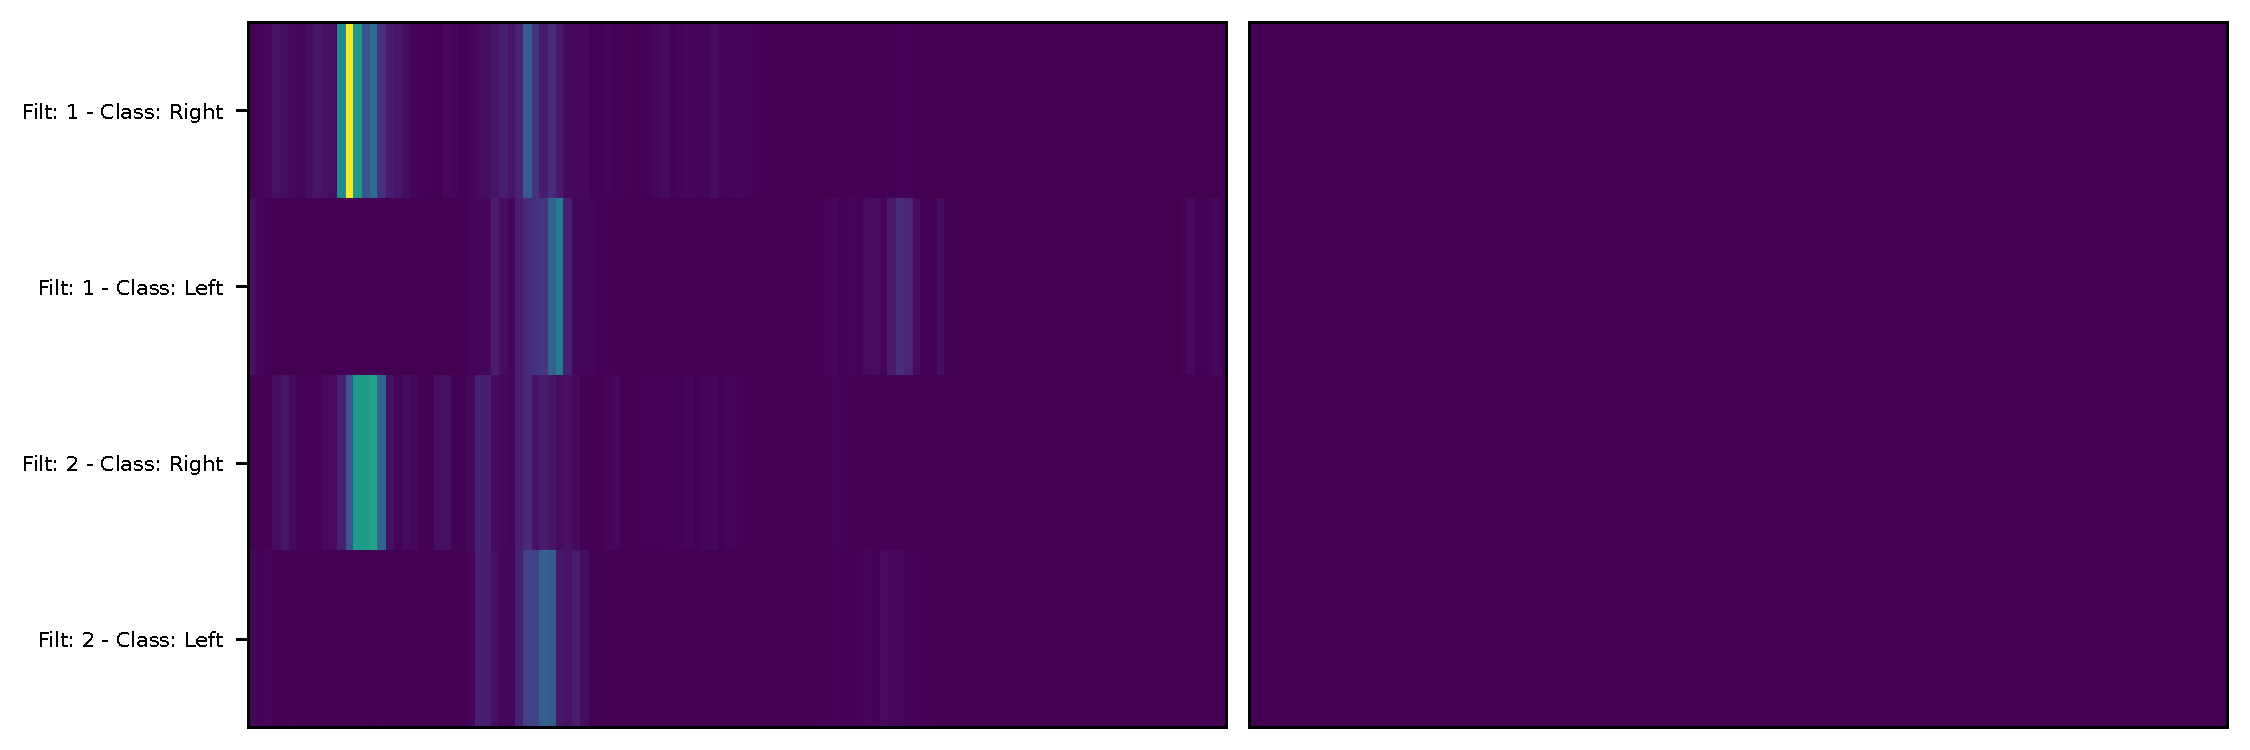
\includegraphics{Figures/Objective_3/subject_4_group_GI.pdf}}} \\

{\rotatebox{90}{\hspace{10mm} \textbf{Subject 42 - G II}}} &
{\resizebox{\kerrwidth}{!}{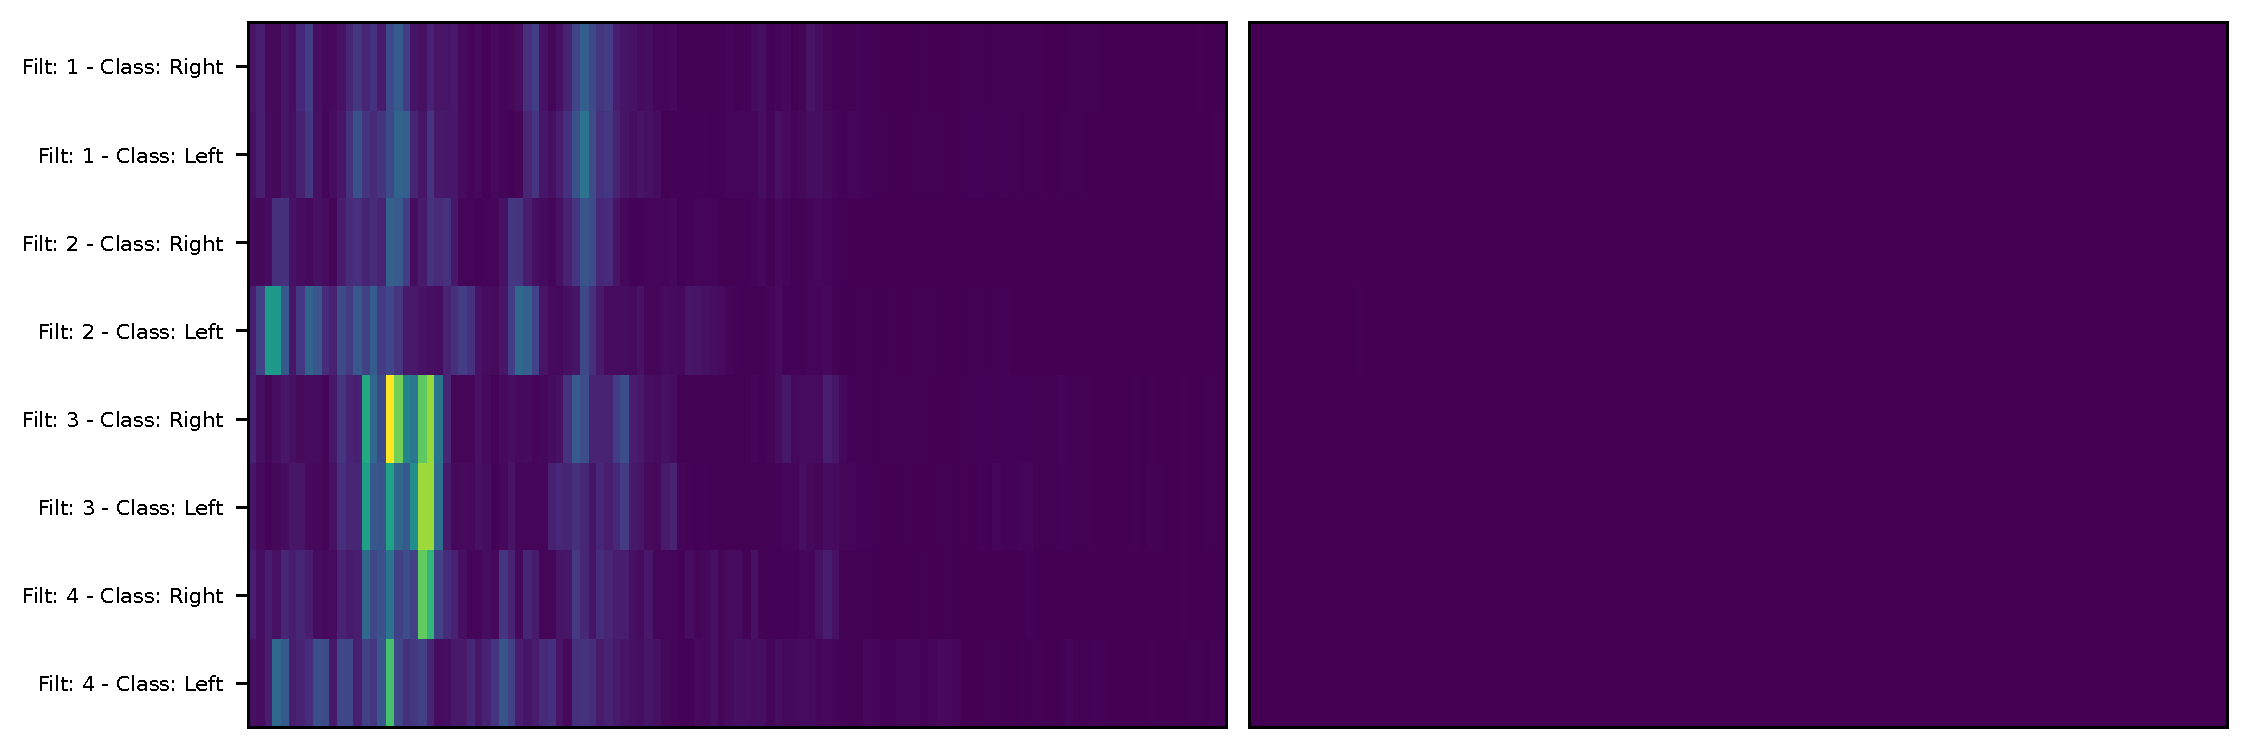
\includegraphics{Figures/Objective_3/subject_42_group_GII.pdf}}} \\

{\rotatebox{90}{\hspace{10mm} \textbf{Subject 51 - G III}}} &
{\resizebox{\kerrwidth}{!}{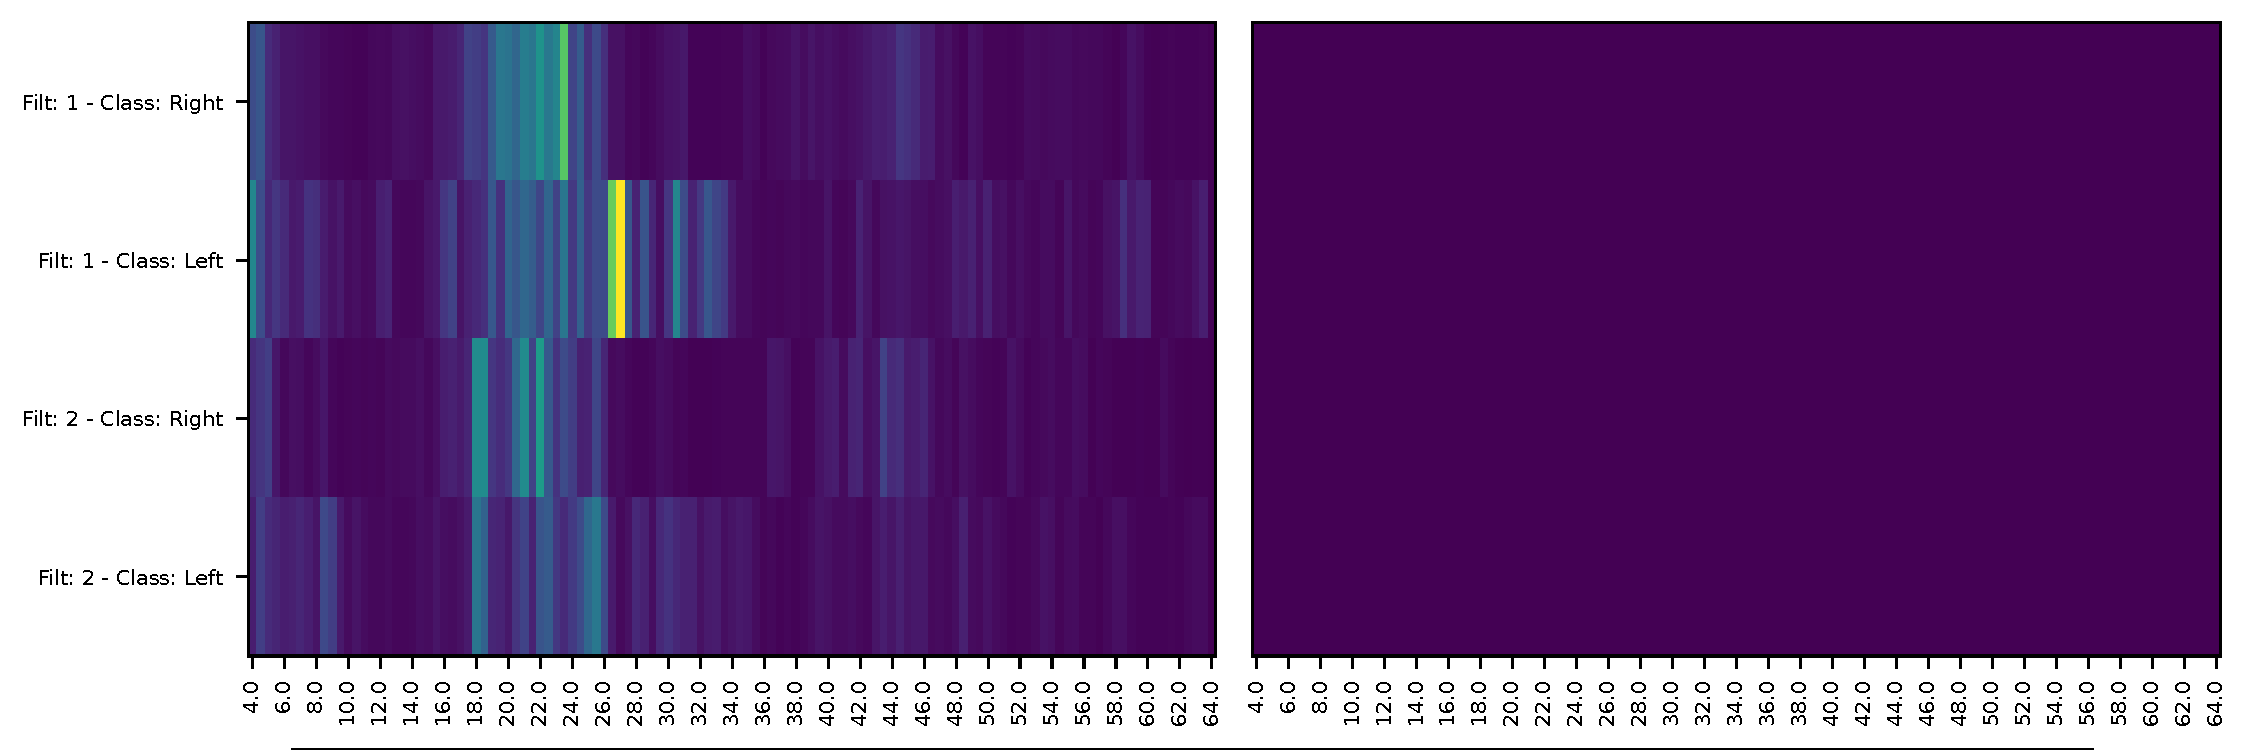
\includegraphics[trim=0 10 0 0, clip]{Figures/Objective_3/subject_51_group_GIII.pdf}}} \\
 & {\hspace{20mm}  \resizebox{0.5\linewidth}{!}{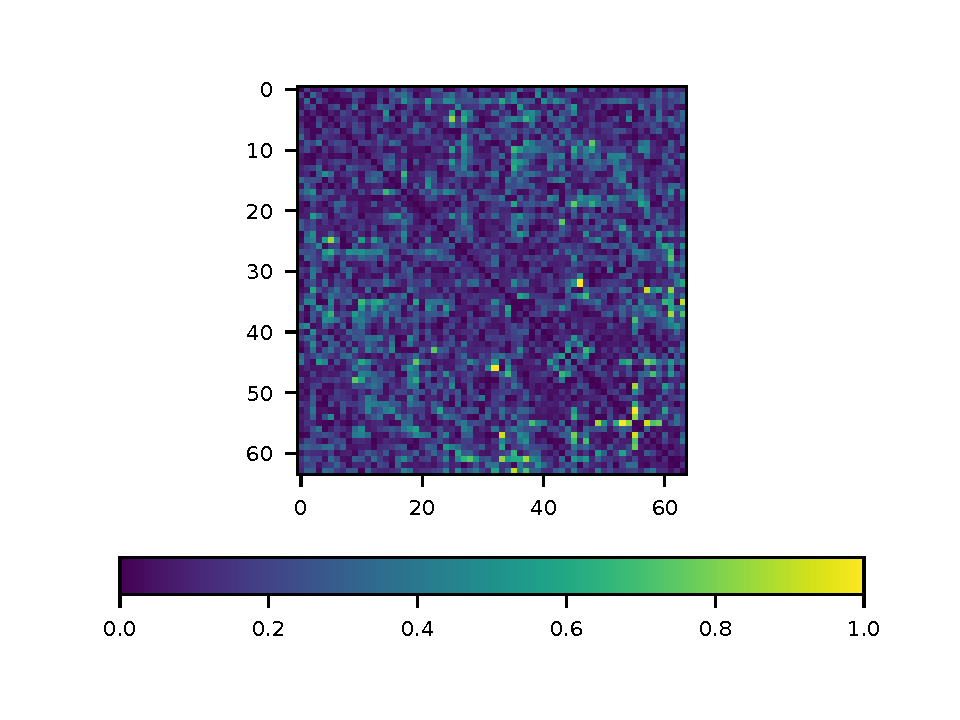
\includegraphics[trim=0 0 0 250, clip]{Figures/Objective_3/colorbar2.pdf}}} &\\
\end{tabular}
\caption{Illustration of the PSD across subjects 4, 42, and 51 from groups I, II, and III, respectively. While Groups I and II display localized and specific frequency band importance for motor tasks, Group III suggests more spread frequencies. Zero cross-label importance across all subjects indicates that the model effectively prevents misclassification but suggests potential overfitting. \label{fig:psd_ind_filt}}
\end{figure}


\section{Summary}

We have developed an interpretable, regularized, end-to-end DL architecture for EEG-based MI-BCI systems called the Interpretable Regularized Kernel Cross-Spectral Functional Connectivity Network (IRKCS-FCnet). This architecture, when combined with a post-hoc and intrinsic interpretability strategy, addresses transparency and interpretation challenges in MI-BCI models, as detailed in \cref{sec:problem3}. We employ the proposed architecture to derive an intrinsic interpretation directly from the weights of the final layer. At the same time, we enhance the cross-information potential in the KCS-FC block to achieve sparser FC connectivities. This effectively removes spurious and nonrelevant connectivities related to the MI task. To facilitate this, we have integrated Renyi's entropy $\alpha=2$ into the cross-entropy loss function, emphasizing the maximization of cross-information potential and increasing the probability of the correct label. Moreover, by employing the average drop score, an effective method to measure interpretability results based on the hierarchical removal of critical features, we can compare regular and plain versions of KCS-FC-based DL architectures. Notably, our IRKCS-FCnet has revealed the contralateral concept of MI in both the right and left-hand classes. This comprehensive interpretability method has deepened our understanding of the operation of the KCS-FC block and has provided helpful insight into the potential further enhancement of the proposed architectures.